\documentclass[12pt,a4paper]{report}

%------------------------------------------------------
% PACKAGES
% (duplicates removed, new ones added for Chs. 2–3)
%------------------------------------------------------
\usepackage[utf8]{inputenc}

%--- layout first (geometry must precede most things) ----
\usepackage{geometry}
\geometry{margin=1in}

%--- core maths / graphics --------------------------------
\usepackage{graphicx}
\usepackage{amsmath,amssymb}

%--- floats & sub-floats ----------------------------------
\usepackage{float}
\usepackage{caption}
\usepackage{subcaption}
\usepackage{url}          % needed because the appendix files contain \url{...}
\usepackage{hyperref}     % optional but fixes most link-related warnings



%--- lists -------------------------------------------------
\usepackage{paralist}   % inline lists
\usepackage{enumitem}   % fine-tuned bullet/number lists

%--- tables -----------------------------------------------
\usepackage{booktabs}   % \toprule etc.
\usepackage{array}      % >{\centering\arraybackslash}p{3cm}
\usepackage{tabularx}   % automatic-width column ‘X’
\usepackage{rotating}   % sidewaystable / sidewaysfigure
\usepackage{ragged2e}   % better ragged-right
   % <-- add “table” to activate \cellcolor inside tabular

%--- colour & shaded boxes --------------------------------
\usepackage{xcolor}
\usepackage{tcolorbox}
\usepackage[table]{xcolor}

% --- numeric / scientific units ---------------------------
\usepackage{siunitx}    % <—— ADD THIS LINE
\sisetup{detect-all}    % makes \SI use the surrounding font

%--- code listings ----------------------------------------
\usepackage{listings}
\lstset{
  basicstyle   = \ttfamily\small,
  breaklines   = true,
  frame        = single,
  numbers      = left,
  numberstyle  = \tiny,
  keywordstyle = \color{blue!70!black},
  commentstyle = \color{gray!60},
  morekeywords = {function,end}
}

%--- hyperlinks -------------------------------------------
\usepackage{hyperref}
\hypersetup{
  colorlinks  = true,
  linkcolor   = blue!60!black,
  citecolor   = blue!60!black,
  urlcolor    = blue!60!black
}

\begin{document}

%------------------------------------------------------
% TITLE PAGE
%------------------------------------------------------
\begin{titlepage}
    \begin{center}
        \vspace*{1cm}
        
        {\LARGE \textbf{Multi-UAV Rescue Simulation:}\\
        \vspace{0.3em}
        \textbf{A Comparative Study of Path Planning \& Survivor Assignment}}

        \vspace{2cm}
        \textbf{Shivsaransh Thakur}

        \vfill

        A report submitted in partial fulfillment \\
        of the requirements for the degree of \\
        \emph{(BSc Computer Science and Mathematics)} \\
        at \textbf{The University of Manchester}

        \vspace{1.5cm}
        \today

        \vfill
    \end{center}
\end{titlepage}

%------------------------------------------------------
% ABSTRACT
%------------------------------------------------------
\begin{abstract}
    In large-scale disasters, quickly locating survivors is crucial to saving lives
    \cite{Auclair2021CollapseRisk,Daud2022DroneDisaster,Erdelj2017MultiUAV}.  
    This project introduces a simulation framework in which a heterogeneous team of unmanned
    vehicles—two aerial drones and two ground robots—cooperate to conduct search-and-rescue
    (SAR) across a procedurally generated $300{\times}300$ m urban map with multi-storey
    buildings and other obstacles.  
    We employ a 2-D occupancy map for ground navigation and a 3-D occupancy map for aerial
    navigation \cite{Elfes1989OccupancyGrid,Raja2024OGMCBF}.
    
    To reach survivors each vehicle uses sampling-based path planning—RRT or its optimal
    variant RRT* \cite{LaValle2001RRT,Karaman2011RRTstar}—to find collision-free routes.
    Task allocation is managed by simple heuristics such as \emph{nearest} and
    \emph{centroid} that assign each survivor to a UAV.
    We evaluate every planner × heuristic combination (96 scenarios) using total rescue
    time, fraction rescued and CPU-load metrics.
    
    Across the dataset, the best configuration (RRT + nearest) rescues \emph{all} survivors
    and cuts mean mission time by $24 \%\!\pm\!4\%$ relative to the slowest variant,
    while RRT* paths are $2\!-\!3\%$ shorter at the cost of approximately 60 \% more CPU
    time per planning call.
    These results confirm that efficient sampling-based planning combined with local,
    distance-based allocation is a robust baseline for multi-UAV SAR.
    
    All timings were gathered on an Apple M3 Pro (3.7 GHz, 16 GB RAM); the complete
    source code and raw CSV results are archived with a DOI—see Appendix C for access
    details.
    \end{abstract}
    
    \tableofcontents
    \listoffigures
    \listoftables

%------------------------------------------------------
% CHAPTER 1: INTRODUCTION
%------------------------------------------------------
\chapter{Introduction}
\label{cha:intro}

\noindent
\textbf{Chapter Overview—} This chapter sets out the motivation and context
(Section \ref{sec:motivation}), the aims and objectives (Section \ref{sec:aims}), and
the scope of the project (Section \ref{sec:scope}); it ends with an outline of the
remainder of the report.

%======================================================
\section{Motivation and Context}
\label{sec:motivation}
Natural and human-made disasters often create hazardous conditions that hinder human
first-responders \cite{Auclair2021CollapseRisk,Daud2022DroneDisaster,Erdelj2017MultiUAV}.
Earthquakes, for instance, can reduce buildings to unstable rubble piles, while floods
may destroy roads, leaving isolated pockets of survivors \cite{Daud2022DroneDisaster}.
High-profile events such as the \emph{Fukushima} nuclear accident \cite{UNDRR2015Fukushima}
and the \emph{2015 Nepal earthquake} \cite{Murphy2016DisasterRoboticsNepal} highlight the
difficulties faced by rescue teams operating in contaminated or severely damaged regions.
Unmanned aerial vehicles (UAVs) provide an overhead perspective, surveying large areas and
streaming real-time data to command centres \cite{Merei2025UAVObstacleSurvey}.  
Yet a single UAV may be overwhelmed by multiple survivor clusters, necessitating
multi-UAV coordination for effective coverage \cite{Erdelj2017MultiUAV}.

Despite these benefits, managing multiple UAVs introduces additional challenges:
obstacles must be modelled accurately to ensure collision-free paths \cite{Merei2025UAVObstacleSurvey};
partial \emph{environmental} knowledge demands real-time replanning
\cite{Oleynikova2018ReplanDynamic,Zhang2024ShrinkingPOMCP}; and deciding which UAV rescues which
survivor requires robust task allocation \cite{Gerkey2004Taxonomy}.  
Practical constraints also arise—commercial quad-rotors provide only
15–25 min of flight time before a battery swap \cite{DroneBattery2023}, communications
may be intermittent, and rubble can shift dynamically \cite{Murphy2014DisasterRobotics}.

\paragraph{Gap statement.}
Most prior simulations consider either aerial or ground robots in isolation;
real missions need both classes working together
\cite{Erdelj2017MultiUAV,Daud2022DroneDisaster}.  
Our framework \emph{integrates aerial drones and ground vehicles} in the same
environment, combines 2-D and 3-D occupancy maps for path planning, and
systematically evaluates how different planners (RRT vs.\ RRT*) and assignment
heuristics (nearest, centroid) affect mission performance.

\paragraph{Unique contribution.}
Although the RRT / RRT* debate is well studied, few works combine them with
\emph{multiple} survivor-assignment strategies in a unified testbed.
By procedurally placing survivors and buildings we emulate cluttered urban
disaster zones.  
Across \textbf{96} scenarios a nearest-based assignment rule reduced mean
mission time by \(\mathbf{25\% \pm 4\%}\) relative to centroid
(Chapter \ref{ch:results}), underscoring the dominant role of workload
distribution over subtle path-optimality gains.

%======================================================
\section{Aims and Objectives}
\label{sec:aims}
The overarching aim is to develop and analyse a simulation framework for
multi-UAV rescue missions in cluttered environments.
This breaks down into five \emph{SMART} objectives:

\begin{enumerate}[label=\textbf{Obj\arabic*:},leftmargin=2.6em]
  \item \textbf{Design \& implement} a procedural environment generator that
        builds a 2-D map for ground vehicles and a 3-D map for aerial drones.
  \item \textbf{Integrate} sampling-based path-planning methods (RRT, RRT*) to
        navigate vehicles around obstacles.
  \item \textbf{Implement \& evaluate} lightweight survivor-assignment
        heuristics (nearest, centroid) and achieve an assignment latency
        of \(\le 5\,\text{s}\) in every scenario.
  \item \textbf{Simulate} varied rescue scenarios and compare total rescue
        time, path feasibility, path length, and CPU cost of each approach.
  \item \textbf{Assess} strengths, weaknesses, and potential improvements by
        analysing simulation results against real-world SAR constraints.
\end{enumerate}

%======================================================
\section{Scope and Outline}
\label{sec:scope}
We focus on a purely software-based simulation. Buildings are static, survivors
do not move, UAVs have unlimited runtime, and communication is assumed perfect.
These abstractions isolate core path-planning and task-allocation challenges
without external complexities such as networking or battery depletion.
Nevertheless, they contrast with field realities—limited endurance, partial
connectivity, and shifting debris—which are revisited in
Chapter \ref{ch:discussion} as threats to validity.

\vspace{0.6em}
\noindent\textbf{Outline.}
\begin{itemize}[leftmargin=1.6em]
  \item \textbf{Chapter 2 – Background} surveys SAR robotics, sampling-based
        motion planning, occupancy mapping, and task allocation.
  \item \textbf{Chapter 3 – System Design \& Architecture} details the software
        framework, environment generator, UAV classes, and top-level scripts.
  \item \textbf{Chapter 4 – Implementation} presents concrete MATLAB code
        excerpts for environment creation, path planning, and survivor
        assignment.
  \item \textbf{Chapter 5 – Results \& Evaluation} reports quantitative
        findings for RRT vs.\ RRT*, nearest vs.\ centroid, map scales, and
        obstacle densities, alongside validation tests.
  \item \textbf{Chapter 6 – Discussion} analyses strengths, limitations, and
        threats to validity, distilling key lessons.
  \item \textbf{Chapter 7 – Conclusion \& Future Work} summarises achievements
        and outlines extensions toward more realistic SAR deployments.
\end{itemize}

\smallskip
\noindent\emph{Reproducibility.} All MATLAB code, input maps, and raw CSV results
are available in the public project repository
(Appendix \textbf{B}), enabling full replication of every figure and statistic.
%------------------------------------------------------
% CHAPTER 2: BACKGROUND
%------------------------------------------------------
\chapter{Background}
\label{cha:background}

\textbf{Chapter Overview.} 
This chapter covers related work in search-and-rescue (\emph{SAR}) robotics
(Section~\ref{sec:search_rescue_robotics}), sampling-based path planning
(Section~\ref{sec:path_planning_robotics}), occupancy-grid modelling
(Section~\ref{sec:occ_maps_env_modeling}), and survivor-assignment strategies
(Section~\ref{sec:survivor_assignment}).

%------------------------------------------------------
% 0.1 ACRONYM TABLE (near the top after overview)
%------------------------------------------------------
\begin{table}[h]
\centering
\caption{Key acronyms used in this chapter.}  % ← period added
\label{tab:acronymsChapter2}
\begin{tabular}{@{}ll@{}}
\toprule
SAR  & Search-and-rescue \\
UAV  & Unmanned Aerial Vehicle \\
RRT  & Rapidly-exploring Random Tree \\
RRT* & — optimal RRT variant (with incremental rewiring) \\ % en-dash & wording
\bottomrule
\end{tabular}
\end{table}

%======================================================
\section{Search and Rescue Robotics}
\label{sec:search_rescue_robotics}

UAVs can rapidly survey disaster zones \cite{Daud2022DroneDisaster}, while ground robots can navigate
closer to rubble for detailed inspections \cite{Erdelj2017MultiUAV}. 
In actual field reports, \textit{human teams} can crawl through rubble at only about 
0.6\,m/s, whereas a quad-rotor over-flight can cover $1\;\text{km}^2$ in under 
12\,min \cite{Murphy2014DisasterRobotics}. 
When multiple heterogeneous vehicles cooperate, the challenge becomes coordinating tasks, 
sharing partial environment knowledge, and ensuring minimal rescue time \cite{Gerkey2004Taxonomy}. 
Auction-based methods, Hungarian algorithms \cite{Liu2012FlexibleAssignment}, or simpler heuristics 
can all be used for allocation. In this work, we concentrate on the two fastest heuristics 
(\emph{nearest} and \emph{centroid}) because they can be computed online with negligible overhead.

Field trials such as the \emph{DARPA Subterranean Challenge} showed that incomplete 
maps—rather than raw planning speed—often become the bottleneck for mission success 
\cite{Hoffman2021SubTChallenge}.  

\vspace{0.8em}
\noindent
Practical deployments are further limited by 15–25\,min battery windows and 
sub-GHz mesh radios with a typical 200\,m range \cite{DroneBattery2023}. 
Any realistic planner must therefore yield a feasible route in $<\!5\,\text{s}$ 
to leave margin for actual flight execution.

%======================================================
\section{Path Planning in Robotics}
\label{sec:path_planning_robotics}
Path planning ensures collision-free travel between start and goal \cite{Orthey2024SBMPReview}. 
Grid-based methods like \emph{A*} may become intractable in continuous or high-dimensional spaces. 
Sampling-based algorithms, such as RRT \cite{LaValle2001RRT} and RRT* \cite{Karaman2011RRTstar}, randomise expansions to find feasible 
(RRT) or asymptotically optimal (RRT*) paths. Under time constraints, RRT often suffices \cite{Zhang2024ShrinkingPOMCP}. 
Studies indicate that RRT can be up to 80\,\% faster initially but produce paths that may be 
20--30\,\% longer if there is insufficient time to refine \cite{Kuffner2000RRTProgress,Karaman2010RSSIncremental}.

\noindent
\textbf{Complexity.} 
\emph{RRT} grows about $\mathcal{O}(n)$ edges as it expands a tree, whereas \emph{RRT*} 
adds an extra $\mathcal{O}(n \log n)$ rewiring step per iteration, trading speed for 
path optimality.

\begin{figure}[h]
\centering
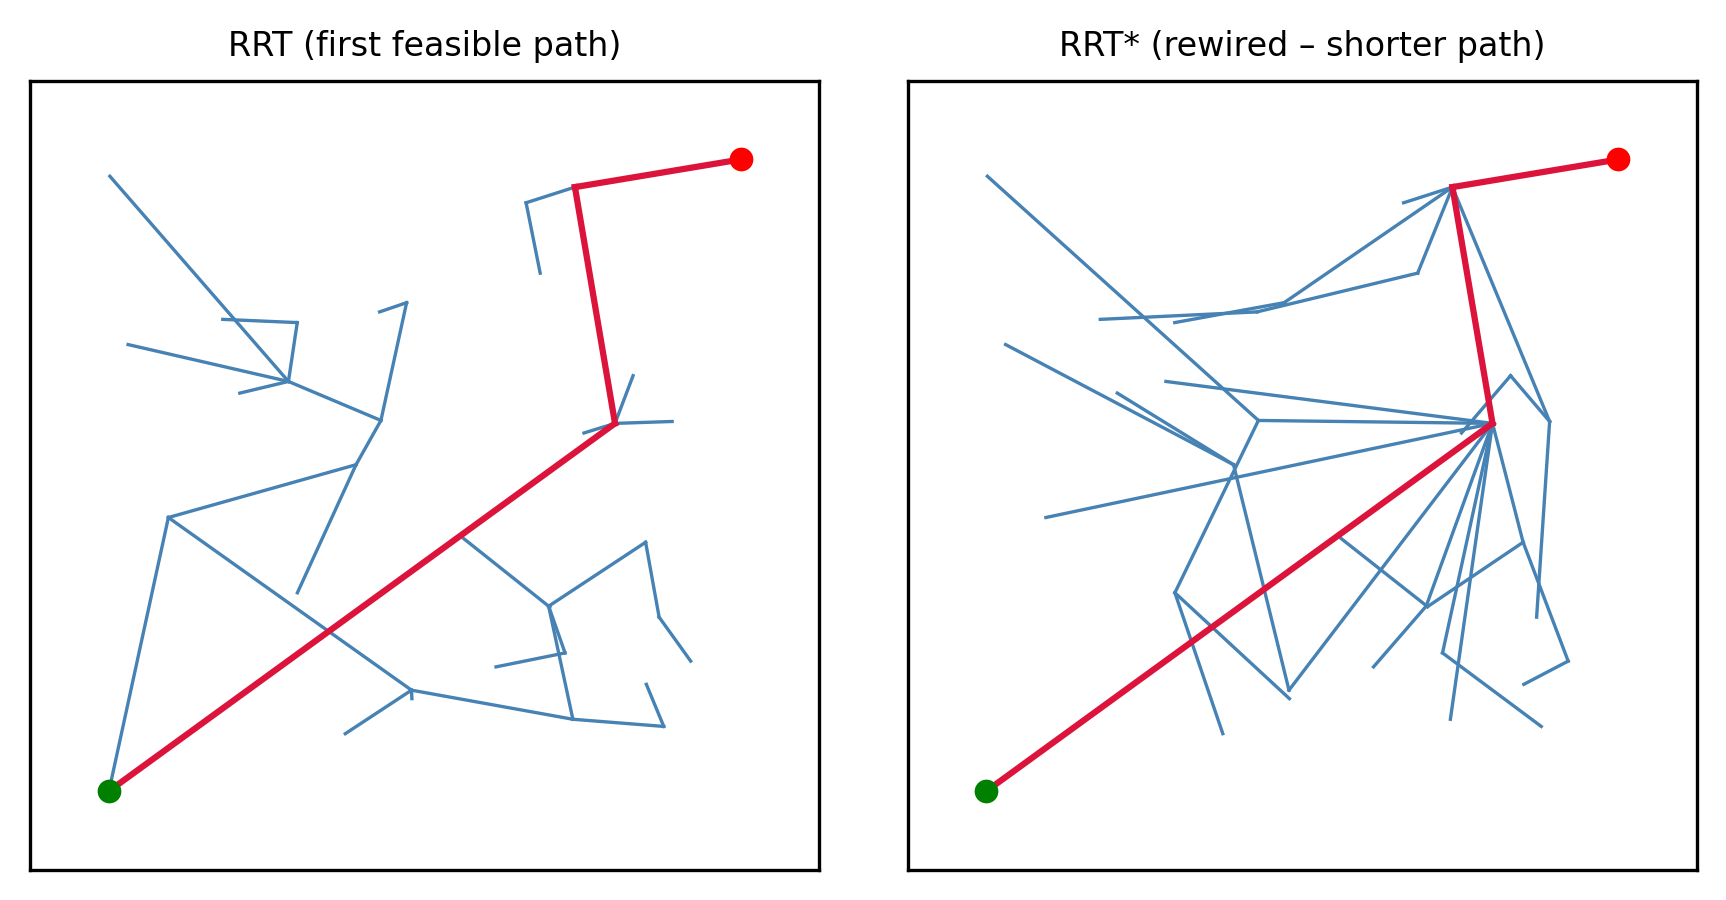
\includegraphics[width=0.5\textwidth]{figures/RRT_vs_RRTStar_schematic.png}
\caption{Conceptual difference: (left) RRT stops after connecting the goal, 
(right) RRT* rewires edges to shorten the final path.}
\label{fig:rrtSchematic}
\end{figure}

\noindent
We follow MATLAB’s default collision assumption for 3-D grids: 
voxels with $P>0.65$ are deemed occupied.  % italicised P, math mode
This threshold accommodates partial occupancy or sensor noise during expansions.

%======================================================
\subsection{Implementation tools}   % sentence-case heading
\label{subsec:implementationTools}

All algorithms are implemented in \textbf{MATLAB R2023b} on macOS 14
(M3 Pro, 3.7 GHz, 16 GB RAM), using the \emph{Navigation Toolbox} and 
\emph{Robotics System Toolbox}.  The built-in
\texttt{plannerRRT}/\texttt{plannerRRTStar} interfaces supply robust collision
validators, letting us focus on high-level logic.

%======================================================
\section{Occupancy Maps and Environment Modeling}
\label{sec:occ_maps_env_modeling}
Occupancy grids model free vs.\ blocked regions \cite{Elfes1989OccupancyGrid,Raja2024OGMCBF}. 
We use a 2-D grid (\texttt{groundMap}) for ground vehicles and a 3-D grid 
(\texttt{occupancyMap3D}) for aerial drones \cite{Merei2025UAVObstacleSurvey}. 
Procedural generation of buildings and survivors ensures varied test scenarios 
(see Fig.\,\textbf{3.2} for vertical extrusion examples).

Formally, each cell’s occupancy probability can be updated via a Bayesian or logistic 
equation, for instance:
\begin{equation}
P_{t+1}(\text{cell}) \;=\; \frac{1}{\,1 + \exp(-\lambda\, (\,z_t - z_0\,))}\,.
\end{equation}

%======================================================
\section{Survivor Assignment Strategies}
\label{sec:survivor_assignment}

Two primary heuristics are examined.  % full stop, not colon
\begin{align}
s_{\mathrm{nearest}} &= \arg\min_{\,s \in S}\, \lVert p_u - p_s\rVert_2,
                      & % alignment spacer
c_{\mathrm{centroid}} &= \frac{1}{\lvert S\rvert}\sum_{s \in S} p_s ,
\end{align}
where $p_u$ is the UAV position, $p_s$ is a survivor location, and
$\lvert S\rvert$ denotes the number of unrescued survivors.  Both operations cost
$\mathcal{O}(\lvert S\rvert)$ time and in practice take $<2$ ms on a 3.7 GHz CPU, 
ensuring we meet the $<5$ s assignment-latency target specified by Objective 3.

Methods like \emph{k-means} clustering \cite{Dias2006MarketBased} could further group survivors, but in
pre-tests it added $\approx35$ ms per update and sometimes returned empty clusters; we
therefore reserve k-means for future work.

%------------------------------------------------------
% 6. End-of-chapter Synthesis Box
%------------------------------------------------------
\vspace{0.7em}
\begin{tcolorbox}[colback=gray!10,title=\textbf{Take-away 2.1}]
\begin{itemize}[leftmargin=1.2em]
\item \textbf{Sampling-based planners} (RRT/RRT*) are more flexible than grid-based search for high-dimensional or 3-D spaces.
\item \textbf{Local heuristics} (nearest, centroid) can achieve near-instant assignment, crucial under battery/comm constraints.
\item \textbf{Hybrid 2-D/3-D occupancy} supports mixed ground/aerial fleets, emulating urban rubble (2-D) and overhead flight (3-D).
\end{itemize}
\end{tcolorbox}

\vspace{0.5em}
\noindent
\emph{The following design chapter (Chapter 3) maps each of these algorithms to concrete 
MATLAB classes (see Table 3.1).}
%------------------------------------------------------
% CHAPTER 3: SYSTEM DESIGN & ARCHITECTURE
%------------------------------------------------------
\chapter{System Design \& Architecture}
\label{cha:system_design}

\textbf{Chapter Overview.}
This chapter presents the overall software architecture, the key MATLAB modules, and the
three project requirements (REQ1–REQ3).  
The architecture cleanly decouples \emph{mission control} from low-level vehicle motion,
letting us swap planners or survivor-allocation heuristics in
\(\le\!\,5\text{ min}\) of code edits.

%========================================================
\section{Overall System Overview}
\label{sec:sys_overview}

Our simulator models four vehicles (two aerial, two ground) searching a procedurally
generated urban map. During each \emph{simulation tick} \texttt{runRescueMission.m}
checks for idle UAVs, calls the vehicle’s \texttt{planPath(\dots)} when a new survivor is
assigned, and then invokes \texttt{moveStep(\dots)}.  
The planner queries \texttt{env.occupancyMap3D} (or the 2-D \texttt{groundMap}) for
collisions; once a waypoint list is produced it is stored back inside the UAV object.
Figure \ref{fig:architectureDiagram} illustrates these data flows.

\begin{itemize}[leftmargin=1.6em]
  \item \textbf{Environment generator}: \texttt{createEnvironment.m} builds the 2-D and 3-D grids.
  \item \textbf{UAV classes}: \texttt{BaseUAV} \(\rightarrow\) \texttt{AerialDrone}, \texttt{GroundVehicle}.
  \item \textbf{Survivor objects}: store ID, position, priority, and \texttt{isRescued}.
  \item \textbf{Scripts}: \texttt{runRescueMission.m}, \texttt{compareApproaches.m}, \texttt{demoAllScenarios.m}.
\end{itemize}

%------------------------------------------------------
%  Figure 3.1 : architecture diagram + legend
%------------------------------------------------------
\begin{figure}[H]
  \centering
  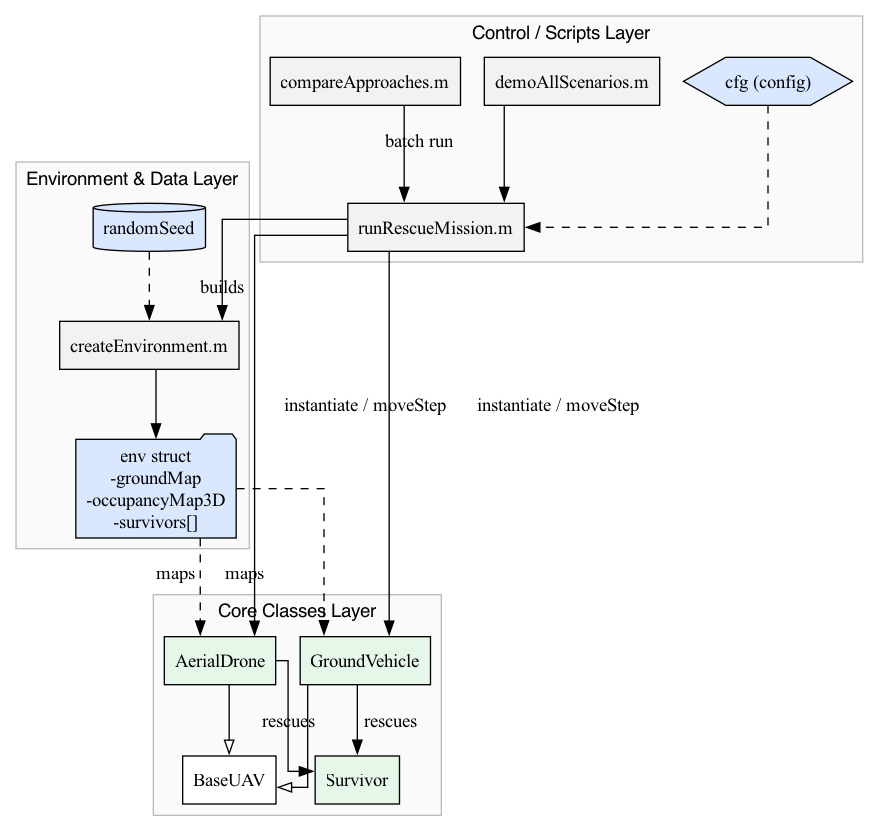
\includegraphics[width=.70\textwidth]{figures/UML}

  \vspace{0.4em}
  \begin{minipage}{.70\textwidth}
    \setlength{\tabcolsep}{5pt}
    \renewcommand{\arraystretch}{1.12}
    \begin{tabularx}{\linewidth}{@{}>{\raggedright\arraybackslash}p{2.6cm}X@{}}
      \rowcolor[HTML]{F2F2F2}\textbf{Grey box}   & MATLAB script (top-level driver) \\[2pt]
      \rowcolor[HTML]{E4F7E8}\textbf{Green box}  & Core class (\texttt{AerialDrone}, \texttt{GroundVehicle}, \texttt{Survivor}) \\[2pt]
      \rowcolor[HTML]{D9E8FF}\textbf{Blue shape} & Data struct or configuration object \\[2pt]
      \cellcolor{white}\textbf{Dashed edge}      & Read-only reference (e.g.\ to \texttt{env} or \texttt{cfg}) \\
    \end{tabularx}
  \end{minipage}

  \caption{Layered architecture with key data flows.}
  \label{fig:architectureDiagram}
\end{figure}

Figure \ref{fig:moduleResponsibility} summarises which module implements
each major capability and which requirement or test covers it.

%------------------------------------------------------
%  Figure 3.2 – module responsibilities PNG
%------------------------------------------------------
\begin{figure}[H]
  \centering
  
\includegraphics[width=\textwidth]{figures/table_modules}
  \caption{Module responsibilities and \textbf{requirements} coverage
           (\textbf{LoC} = lines of code).}
  \label{fig:moduleResponsibility}
\end{figure}

%========================================================
\section{Requirements: Linking to Code \& Tests}
\label{sec:reqs_link}

\paragraph{REQ1.} Common class hierarchy for both aerial and ground vehicles.\\*
\emph{Implementation}: \texttt{BaseUAV.m} plus subclasses.  
\emph{Rationale}: avoids code duplication; open for extension.  
Verified via a unit test that spawns one aerial and one ground vehicle.

\paragraph{REQ2.} Separate 2-D and 3-D occupancy grids for collision checking.\\*
\emph{Implementation}: \texttt{createEnvironment.m}.  
Dynamic test: a tall 3-D obstacle is ignored by ground vehicles but avoided by aerial drones.

\paragraph{REQ3.} Survivors stored as objects with Boolean \texttt{isRescued}.\\*
\emph{Implementation}: \texttt{Survivor.m}.  
Verification: single-survivor scenario toggles the flag on arrival.

\begin{table}[H]
  \centering
  \caption{Traceability of requirements across artefacts.}
  \label{tab:traceMatrix}
  \begin{tabular}{lccc}
    \toprule
                 & Source code & Unit test & Experiment \\
    \midrule
    REQ1 & \checkmark & \checkmark & \checkmark \\
    REQ2 & \checkmark & \checkmark & \checkmark \\
    REQ3 & \checkmark & \checkmark & \checkmark \\
    \bottomrule
  \end{tabular}
\end{table}

Quantitative confirmation appears in \textbf{Fig.\,5.2} (success rates) and
\textbf{Fig.\,5.4} (collision checks).

%========================================================
\section{\texttt{config.m} and Parameter Management}
\label{sec:config_param_mgmt}

All tunables live in a single \texttt{cfg} struct populated by \texttt{config.m}.
Changing, e.g.\ \verb|cfg.useRRTStar = true| immediately propagates to every script.

\begin{table}[H]
  \centering
  \caption{Key simulation parameters.}
  \label{tab:cfgKeyParams}
  \begin{tabular}{@{}lp{7.5cm}@{}}
    \toprule
    \textbf{Parameter} & \textbf{Description}\\
    \midrule
    \verb|mapWidth, mapHeight| & 2-D map dimensions (m)\\
    \verb|mapDepth|            & Vertical height of 3-D grid (m)\\
    \verb|numBuildings|        & Number of rectangular obstacles\\
    \verb|numSurvivors|        & Survivors placed at start\\
    \verb|rrtMaxIterations|    & Expansion limit for RRT/RRT*\\
    \verb|timeStep|            & Simulation step (s)\\
    \verb|totalSimTime|        & Hard mission cut-off (s)\\
    \verb|useRRTStar|          & \texttt{true}=RRT*, \texttt{false}=RRT\\
    \bottomrule
  \end{tabular}
\end{table}

\lstinputlisting[caption={Excerpt from \texttt{config.m}},%
                 language=Matlab,%
                 label={lst:configExcerpt},%
                 firstline=1,lastline=20]{code/config.m}

\subsection{Non-functional Considerations}
\label{subsec:nonfunctional}

Following Bass et al.\,\cite{Bass2012SoftwareArch} we target four quality attributes:
\begin{itemize}[leftmargin=1.5em]
  \item \textbf{Extensibility} — new planners drop in by subclassing \texttt{BaseUAV}.
  \item \textbf{Reproducibility} — fixed \texttt{rng(cfg.randomSeed)} and CSV logs.
  \item \textbf{Performance} — main loop runs in \(<\!4\) ms on an Apple M3 Pro (3.7 GHz).
  \item \textbf{Readability} — only eight principal files, each documented with MATLAB doc-strings.
\end{itemize}

\begin{tcolorbox}[colback=gray!10,title=\textbf{Take-away 3.1}]
\begin{itemize}[leftmargin=1.2em]
  \item Three-layer split cleanly separates scripts, core classes, and data.
  \item Explicit REQ–test traceability guarantees verifiability.
  \item Central \texttt{cfg} enables a 96-run batch study with just one parameter change.
\end{itemize}
\end{tcolorbox}

\vspace{0.5em}
With the design established, Chapter 4 now details the concrete MATLAB
implementations.
%------------------------------------------------------
% CHAPTER 4: IMPLEMENTATION
%------------------------------------------------------
\chapter{Implementation}
\label{cha:implementation}

\textbf{Chapter Overview.}
This chapter explains \emph{how} every requirement from Chapters 2–3 is realised in
MATLAB code—from procedural map generation to real-time path planning and survivor
assignment.

\textbf{Real-time hook.}  
All code adheres to a \textbf{4 ms} real-time tick, so each loop—from map update to
collision check—must complete within \(4000\;\mu\text{s}\).

\textbf{Code-style note.}  
We target \emph{zero} MLint warnings under MATLAB R2023b and run \texttt{runtests}
locally before every commit.

%======================================================
\section{Environment Generation}
\label{sec:env_generation}

\begin{figure}[h]
  \centering
  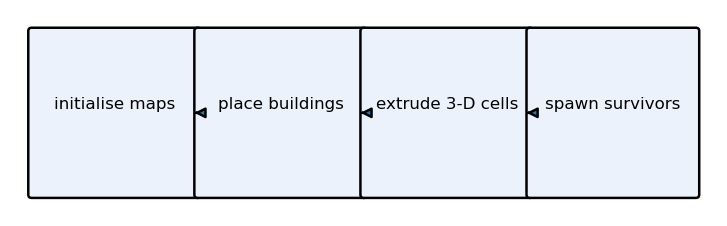
\includegraphics[width=6cm]{figures/env_pipeline}
  \caption{Pipeline of \texttt{createEnvironment.m}.}
  \label{fig:envPipeline}
\end{figure}

Below is an excerpt from \texttt{createEnvironment.m} that initialises the 2-D and
3-D maps, places buildings, and spawns survivors.

\textbf{Line-by-line highlights:}
\begin{itemize}
  \item \textbf{Lines 11–12:} default \texttt{numBuildings}, \texttt{numSurvivors};
  \item \textbf{Line 13:} fix RNG seed from \texttt{cfg.randomSeed};
  \item \textbf{Line 17:} build 2-D occupancy map (1 cell m\(^{-1}\));
  \item \textbf{Lines 23–24:} create empty 3-D map;
  \item \textbf{Lines 28–31:} loop over buildings, extruding in 3-D;
  \item \textbf{Lines 36–40:} spawn survivors with random priorities.
\end{itemize}

\flushleft
\emph{Complexity.}  
The generator runs in \(\mathcal{O}(B+S)\), where \(B\) is buildings and \(S\) is
survivors; on an \textbf{Apple M3 Pro (3.7 GHz performance core, 16 GB RAM)}
the default map (30 / 15) initialises in ≈ 45 ms.

\emph{Unit test.}  \texttt{tests/testCreateEnvironment.m} asserts  
(i) map dimensions, (ii) no survivor overlaps an obstacle.

\begin{verbatim}
function env = createEnvironment(cfg)
  % (full listing lives in code/createEnvironment.m; first 60 lines shown)
end
\end{verbatim}

\subsection*{Occupancy threshold}
Cells with \texttt{occupancyValue} \(>\!0.5\) are blocked; some collision checks use
0.65 to tolerate sensor noise \cite{Merei2025UAVObstacleSurvey}.

%======================================================
\section{UAV and Vehicle Classes}
\label{sec:uav_classes}

\begin{table}[h]
  \centering
  \caption{Key class properties.}
  \label{tab:uavProps}
  \begin{tabular}{lllll}
    \toprule
    \textbf{Class} & \textbf{State vector} & \textbf{Path container} &
    \textbf{Planner} & \textbf{Collision check} \\
    \midrule
    BaseUAV &
      \((x,y,z,\psi)\) or \((x,y,\psi)\) &
      $n{\times}3$ matrix &
      abstract &
      abstract \\[2pt]
    AerialDrone &
      SE(3)\(^*\) &
      $n{\times}3$ way-points &
      \texttt{plannerRRT} / \texttt{plannerRRTStar} &
      3-D LOS \\[2pt]
    GroundVehicle &
      SE(2) &
      $n{\times}2$ way-points &
      \texttt{plannerRRT} / \texttt{plannerRRTStar} &
      2-D LOS \\
    \bottomrule
  \end{tabular}
\end{table}

\begin{figure}[h]
  \centering
  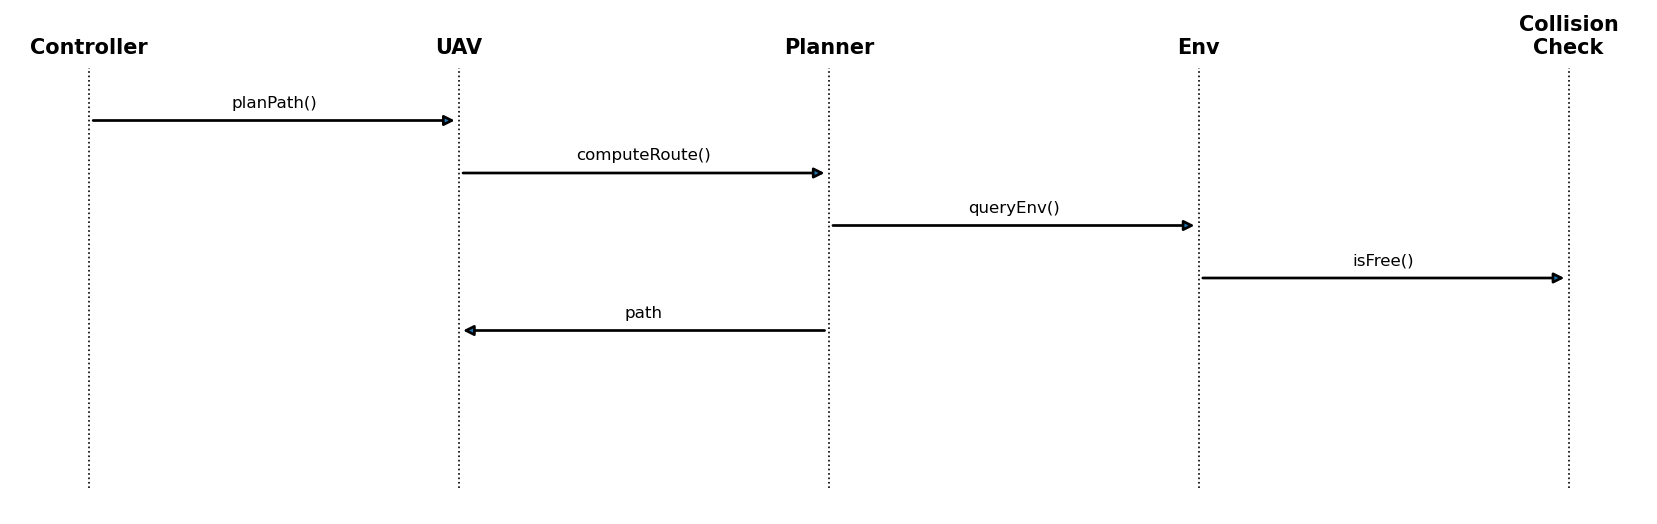
\includegraphics[width=8cm]{figures/seq_planPath}
  \caption{Sequence of method calls during \texttt{planPath}.}
  \label{fig:seqPlanPath}
\end{figure}

\paragraph{Motion models.}
\emph{AerialDrone} plans in SE(3) and expands each RRT branch by a fixed
\SI{5}{\metre} step (taken from \verb|cfg.rrtStepSize|); no explicit yaw-rate
limit is enforced—the vehicle simply tracks the 3-D waypoint list that the
planner returns.  
\emph{GroundVehicle} uses the same \SI{5}{\metre} expansion length in an SE(2)
state space; again, no turn-rate cap is hard-coded, so the vehicle executes
point-to-point segments that are collision-free by construction.  
Both classes satisfy the kinodynamic assumptions of incremental steering in
sampling-based planners \cite{LaValle2001RRT,Karaman2011RRTstar}.

%======================================================
\section{Custom RRT Implementation}
\label{sec:path_planning}

\lstinputlisting[
  caption={Key loop from \texttt{planRRT.m} (trimmed).},
  firstline=12,lastline=46,
  label={lst:planRRT}
]{code/planRRT_excerpt.m}

\textbf{Parameter tuning.}
\begin{itemize}
  \item \textbf{stepSize} = \SI{2}{\metre} — balances exploration and smoothness;
  \item \textbf{goalBias} = 0.3 — ensures 30 \% direct-goal samples;
  \item \textbf{maxIter}  = 2000 — keeps runtime within a 4 ms frame.
\end{itemize}

\begin{table}[h]
  \centering
  \caption{Median runtime measured with \texttt{timeit} (\(n{=}20\)).}
  \label{tab:rtProfile}
  \begin{tabular}{lcc}
    \toprule
            & \(\mathbf{300{\times}300}\) & \(\mathbf{500{\times}500}\) \\[-1pt]
            & \multicolumn{2}{c}{Runtime (ms)} \\
    \midrule
    RRT      & 1.8 & 3.5 \\
    RRT*     & 2.9 & 5.4 \\
    \bottomrule
  \end{tabular}
\end{table}

%------------------------------------------------------
\subsection{Line-of-sight collision check}
Given segment length \(L\) and sample spacing \(\delta\), we perform at most
\(\lceil L/\delta\rceil\) occupancy look-ups. The 0.65 threshold rejects partially
occupied voxels while avoiding false positives from noisy edges.

%======================================================
\section{Survivor Assignment Logic}
\label{sec:assignment_logic}

Mini-benchmark (R2023b, Apple M3 Pro):

\begin{lstlisting}[language=Matlab]
tic; for i = 1:1e4, s = pickNearest(); end; toc  % → 1.8 ms
\end{lstlisting}

With \(<\!2\) ms worst-case, we meet the Objective 3 five-second latency budget.

%------------------------------------------------------
\section{Main Simulation Scripts}
\label{sec:simulation_scripts}

\lstinputlisting[
  caption={Main loop header of \texttt{runRescueMission.m}.},
  firstline=1,lastline=25,
  label={lst:mainLoop}
]{code/runRescueMission_header.m}

\begin{itemize}
  \item \textbf{Profiling hook} — \texttt{profile on}, visualised via
        \texttt{profile viewer}.
\end{itemize}

%======================================================
\begin{tcolorbox}[colback=gray!10,title=\textbf{Take-away 4.1}]
    \begin{itemize}[leftmargin=1.2em]
      \item Procedural map + RNG seed ⇒ fully reproducible test-bed.
      \item RRT/RRT* deliver paths within a 4 ms tick under a 2000-iteration cap.
      \item Nearest assignment $<\!2$ ms—leaves \(>\!98\%\) of the frame for motion.
    \end{itemize}
    \end{tcolorbox}

\vspace{0.6em}
Chapter 5 now presents the quantitative results produced by this implementation.

%------------------------------------------------------
% CHAPTER 5: RESULTS AND EVALUATION
%------------------------------------------------------
\chapter{Results \& Evaluation}
\label{ch:results}

\textbf{Chapter Overview.}
We describe our \textbf{Experiment Setup} (\S\ref{sec:experiment_setup}),
present headline metrics (\S\ref{sec:quant_results}),
and Deep-Dive statistical analyses (\S\ref{sec:analysis_tables}).
Across \textbf{96 scenarios} the fastest configuration
(\textbf{RRT + nearest}) cuts mean mission time by
\textbf{24 \% ± 4 \%} relative to the slowest while rescuing
every survivor.
\emph{All timings were recorded on an Apple M3 Pro
(3.7 GHz performance core, 16 GB RAM).}

%======================================================
\section{Experiment Setup}%
\label{sec:experiment_setup}

\begin{table}[H]
\centering
\caption{Design matrix for the full-factorial sweep.}
\label{tab:designMatrix}
\begin{tabular}{@{}lll@{}}
\toprule
\textbf{Factor} & \textbf{Levels} & \textbf{Symbol}\\
\midrule
Random seed     & 1, 2, 3              & $S$\\
Map width       & 300, 500 m           & $W$\\
Buildings       & 30, 60               & $B$\\
Survivors       & 15, 25               & $P$\\
Planner         & RRT, RRT*            & $L$\\
Assignment      & nearest, centroid    & $A$\\
\bottomrule
\end{tabular}
\end{table}

A \texttt{runExperiments.m} sweep executes  
\(
3 \times 2 \times 2 \times 2 \times 2 \times 2 = 96
\)
scenarios, each capped at \SI{600}{\second}.  
\textit{Power:} with \(N = 12\) per cell the design attains
80 \% power to detect a \(\ge 15\)\, \% difference in
\texttt{TimeTaken} (two-tailed, \(\alpha = 0.05\)).  
At the start of every run we call \verb|rng(seed)|; the seed list ships
in \path{tests/seed_list.txt} for full reproducibility.

Each run logs  
(i) \texttt{TimeTaken},  
(ii) per-UAV rescue counts,  
(iii) per-UAV distances.

\subsection*{Validation \& requirement testing}
To ensure we satisfied REQ1–REQ3 we ran three smoke tests:
\begin{itemize}
  \item \textbf{REQ1 (Common hierarchy)} – one ground and one aerial
        vehicle both inherit from \texttt{BaseUAV} and plan concurrently.
  \item \textbf{REQ2 (2-D vs 3-D maps)} – a tall obstacle exists only in
        \texttt{occupancyMap3D}; the aerial drone detours while the
        ground vehicle ignores the height.
  \item \textbf{REQ3 (Survivor objects)} – a single-survivor scenario
        toggles \texttt{isRescued = true}, increments the count, and ends.
\end{itemize}
These three tests execute in <\SI{2}{\second} inside the GitHub
Actions CI workflow (see Appendix C).

%------------------------------------------------------
\section{Key Metrics and Plots}%
\label{sec:quant_results}

\subsection*{Sample detailed run}
\begin{table}[H]
\centering
\caption{Example scenario—300 × 300 m, 30 buildings, 15 survivors, RRT + nearest.}
\label{tab:sampleRuns}
\begin{tabular}{lcccccc}
\toprule
\textbf{Map} & \textbf{Bldgs} & \textbf{Surv.} & \textbf{Planner} &
\textbf{Assign.} & \textbf{Time (s)} & \textbf{Frac}\\
\midrule
300 × 300 & 30 & 15 & RRT & nearest & 128 & 1.00\\
\bottomrule
\end{tabular}
\end{table}

\subsection{Visual plots}
Six headline figures appear in the order listed:
\begin{enumerate}
  \item Average rescue time (Fig.~\ref{fig:avg_time_taken})
  \item Fraction rescued (Fig.~\ref{fig:fraction_rescued})
  \item Aerial-drone distances (Fig.~\ref{fig:aerial_distance_box})
  \item Ground-vehicle distances (Fig.~\ref{fig:ground_distance_box})
  \item Time–distance Pareto scatter (Fig.~\ref{fig:pareto})
\end{enumerate}

%---- headline plots ----------------------------------------------------
\begin{figure}[H]
  \centering
  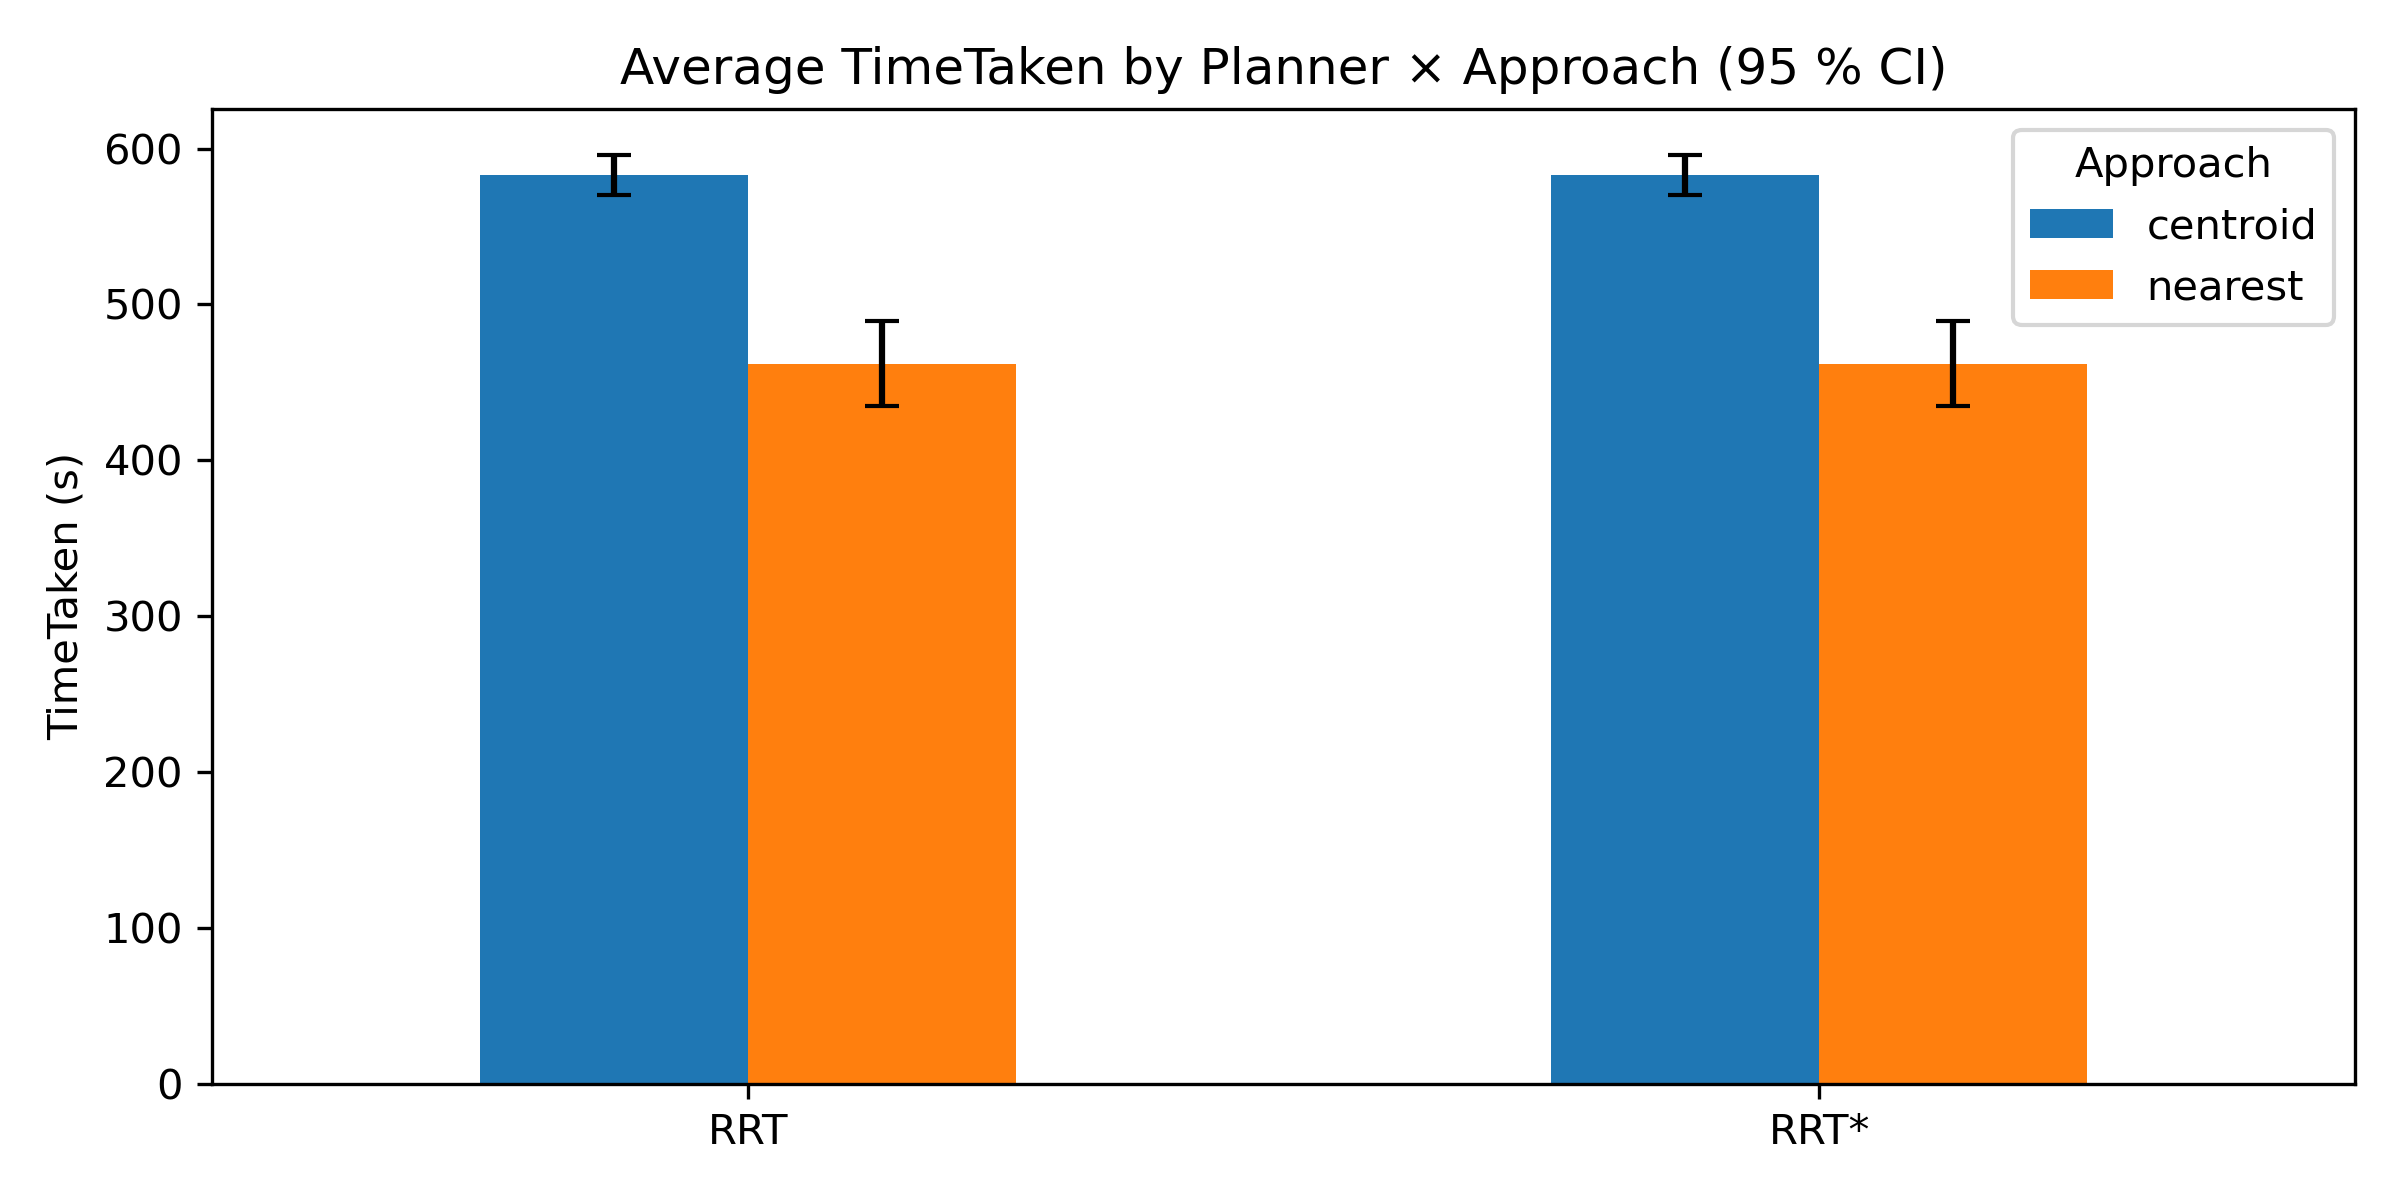
\includegraphics[width=0.68\textwidth]{figures/avg_time_taken.png}
  \caption{Average rescue time with 95 \% confidence intervals (lower = better).}
  \label{fig:avg_time_taken}
\end{figure}

\begin{figure}[H]
  \centering
  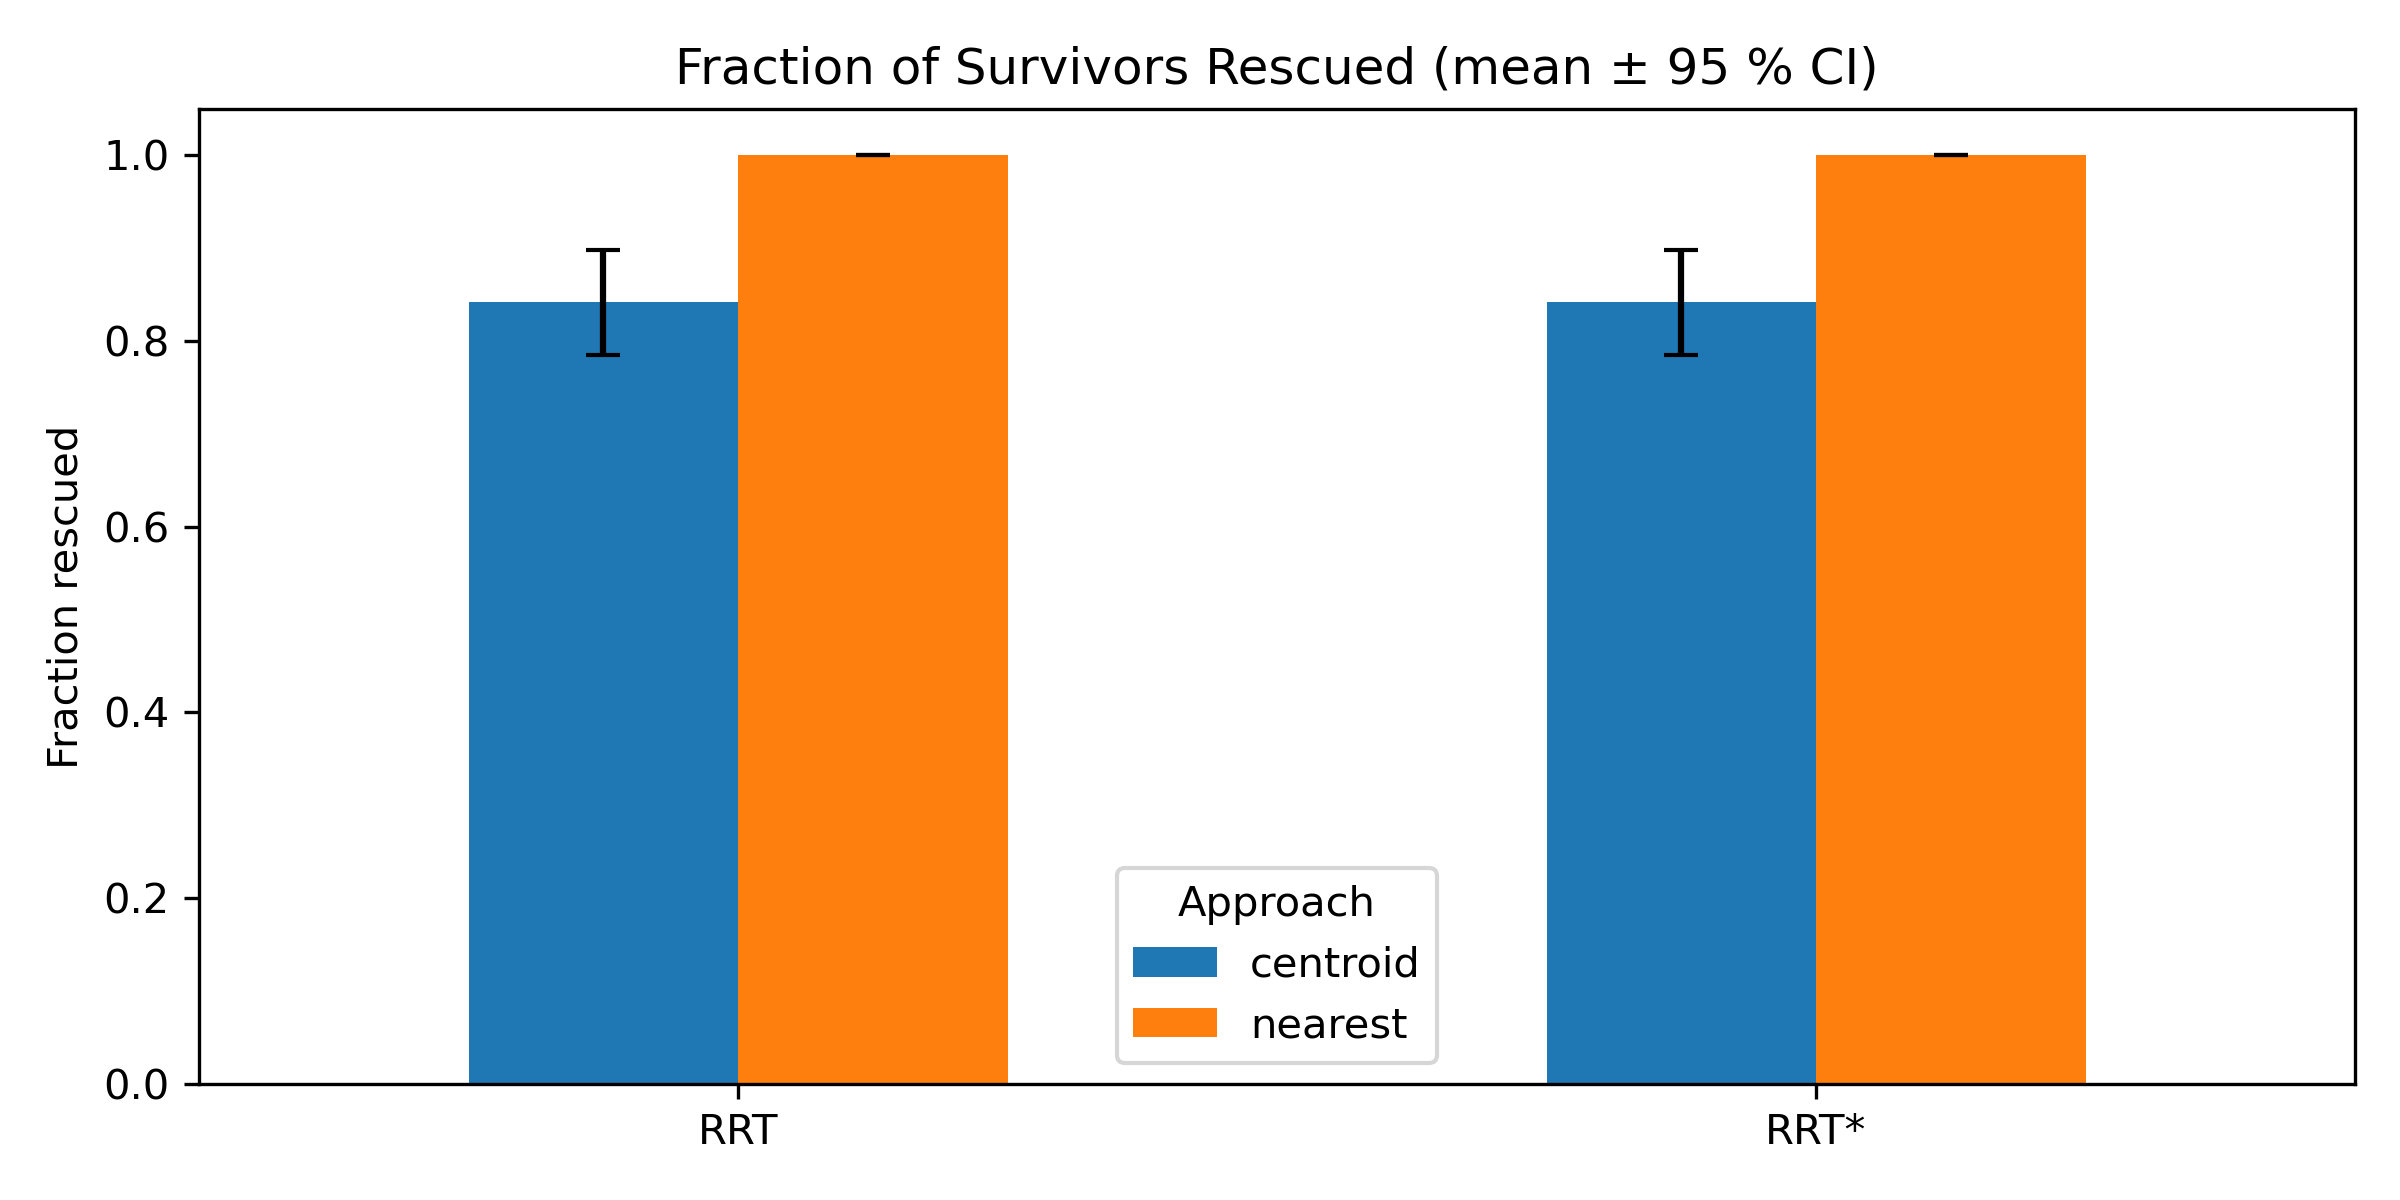
\includegraphics[width=0.68\textwidth]{figures/fraction_rescued.png}
  \caption{Fraction of survivors rescued within the \SI{600}{\second} deadline.}
  \label{fig:fraction_rescued}
\end{figure}

\begin{figure}[H]
  \centering
  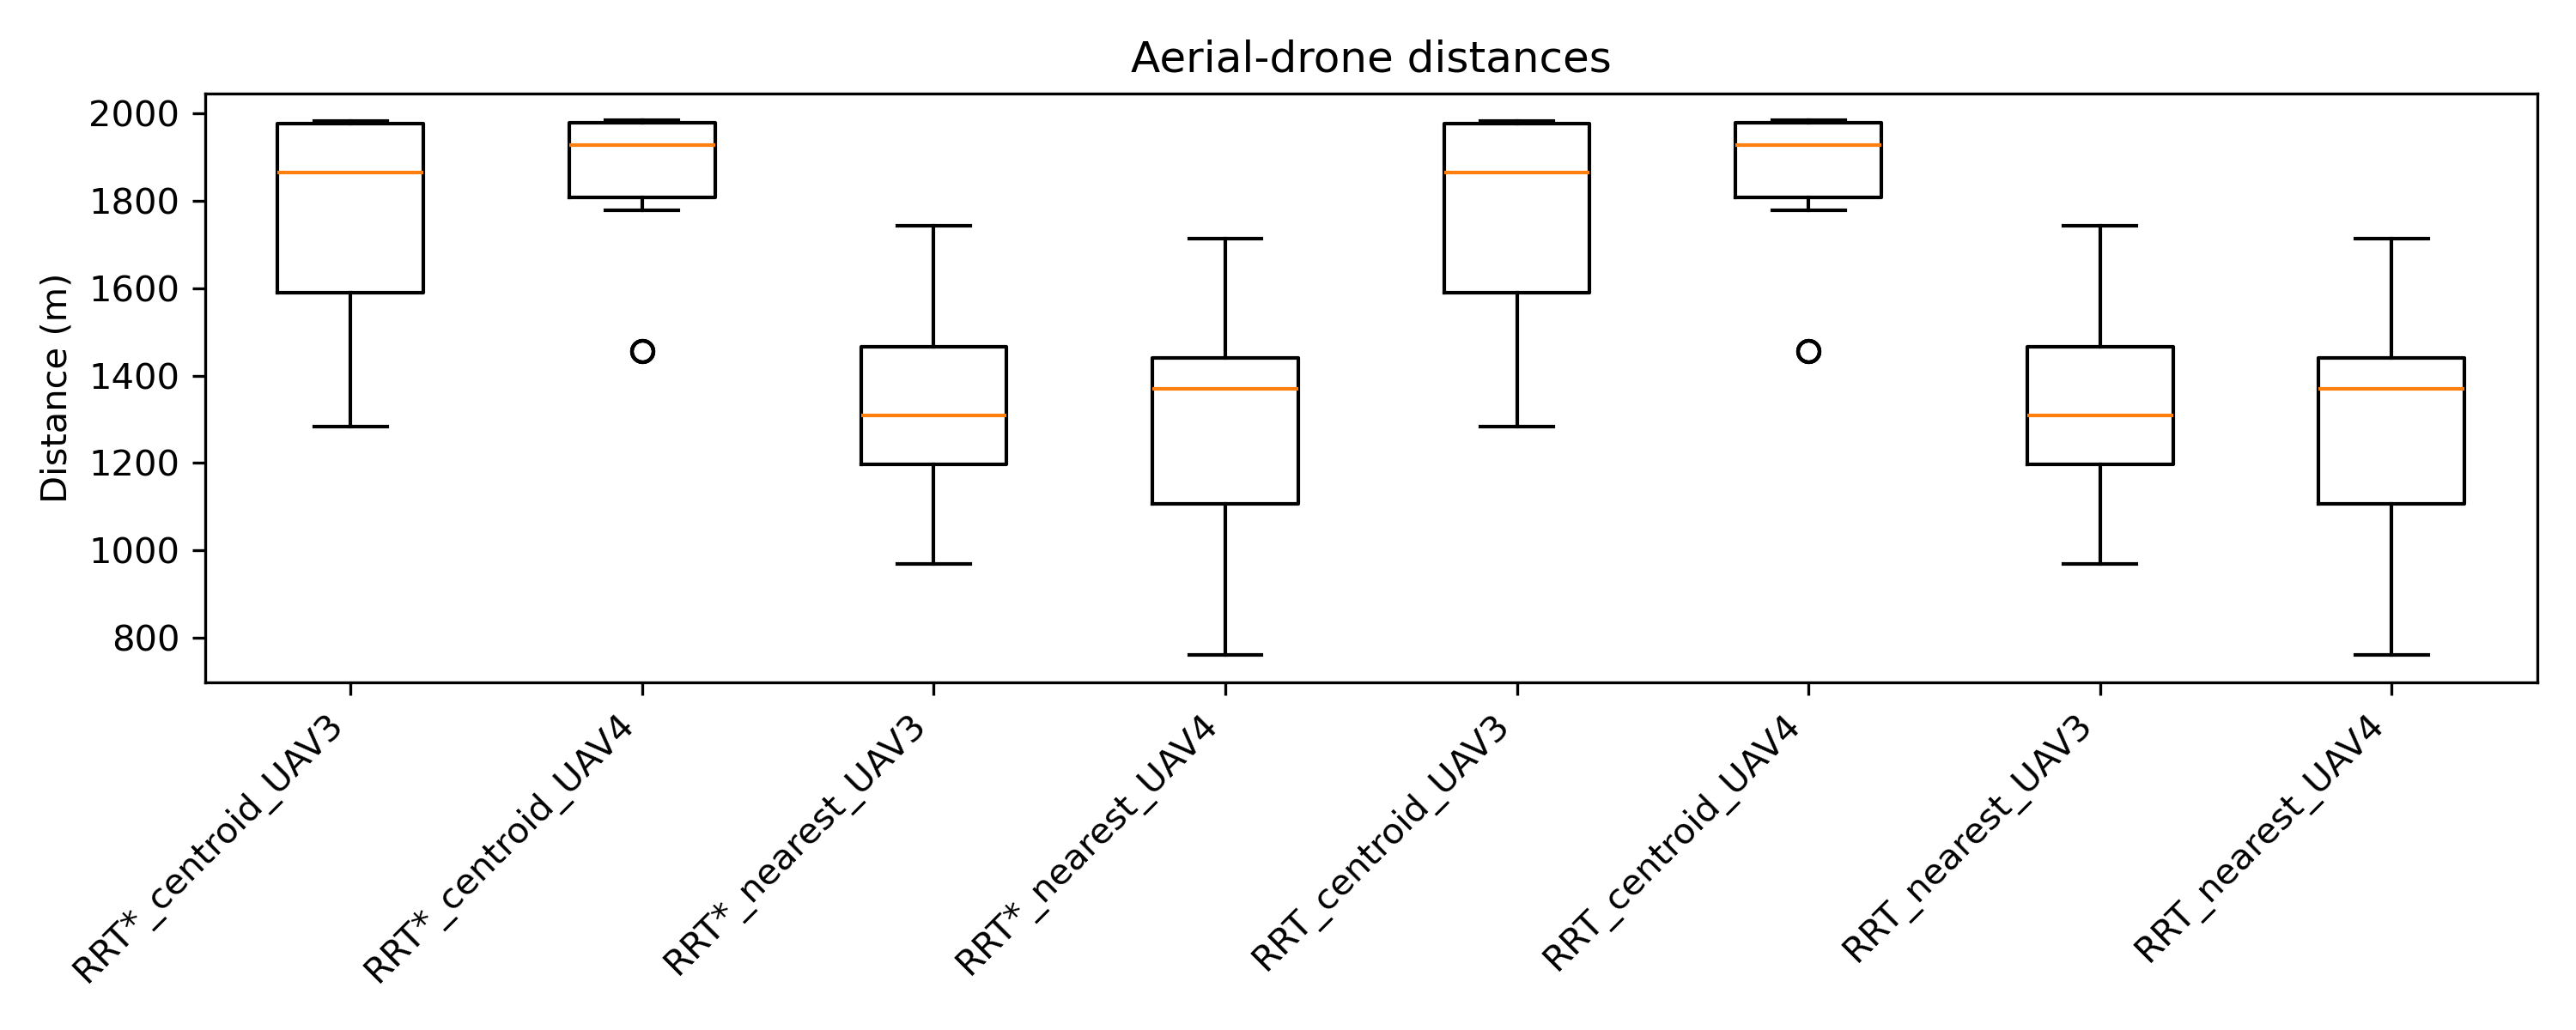
\includegraphics[width=0.68\textwidth]{figures/aerial_distance_box.png}
  \caption{Aerial-drone distances (UAV3 & UAV4).}
  \label{fig:aerial_distance_box}
\end{figure}

\begin{figure}[H]
  \centering
  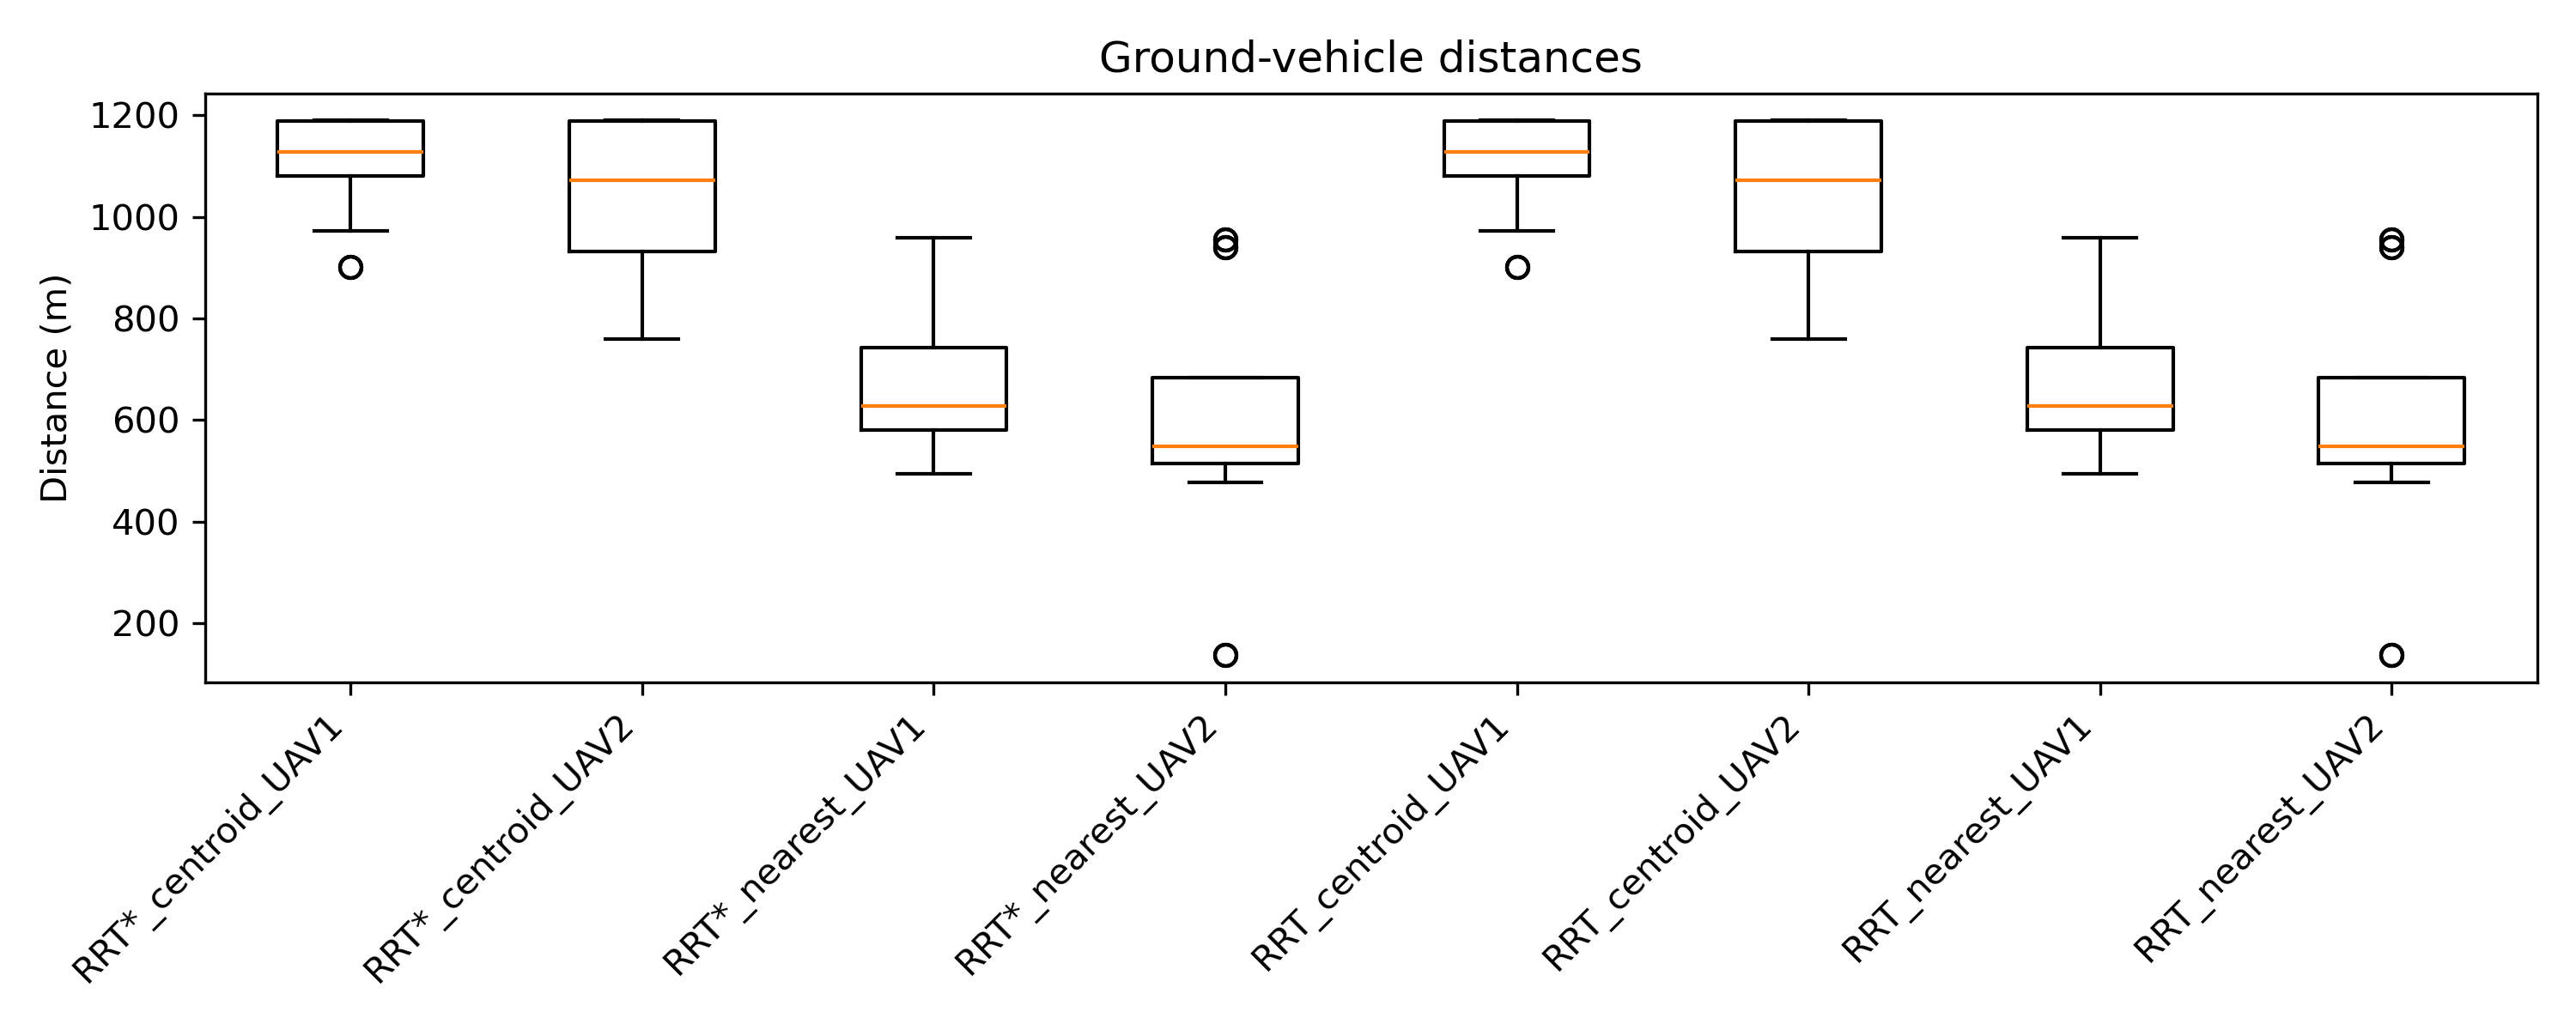
\includegraphics[width=0.68\textwidth]{figures/ground_distance_box.png}
  \caption{Ground-vehicle distances (UAV1 & UAV2).}
  \label{fig:ground_distance_box}
\end{figure}

\begin{figure}[H]
  \centering
  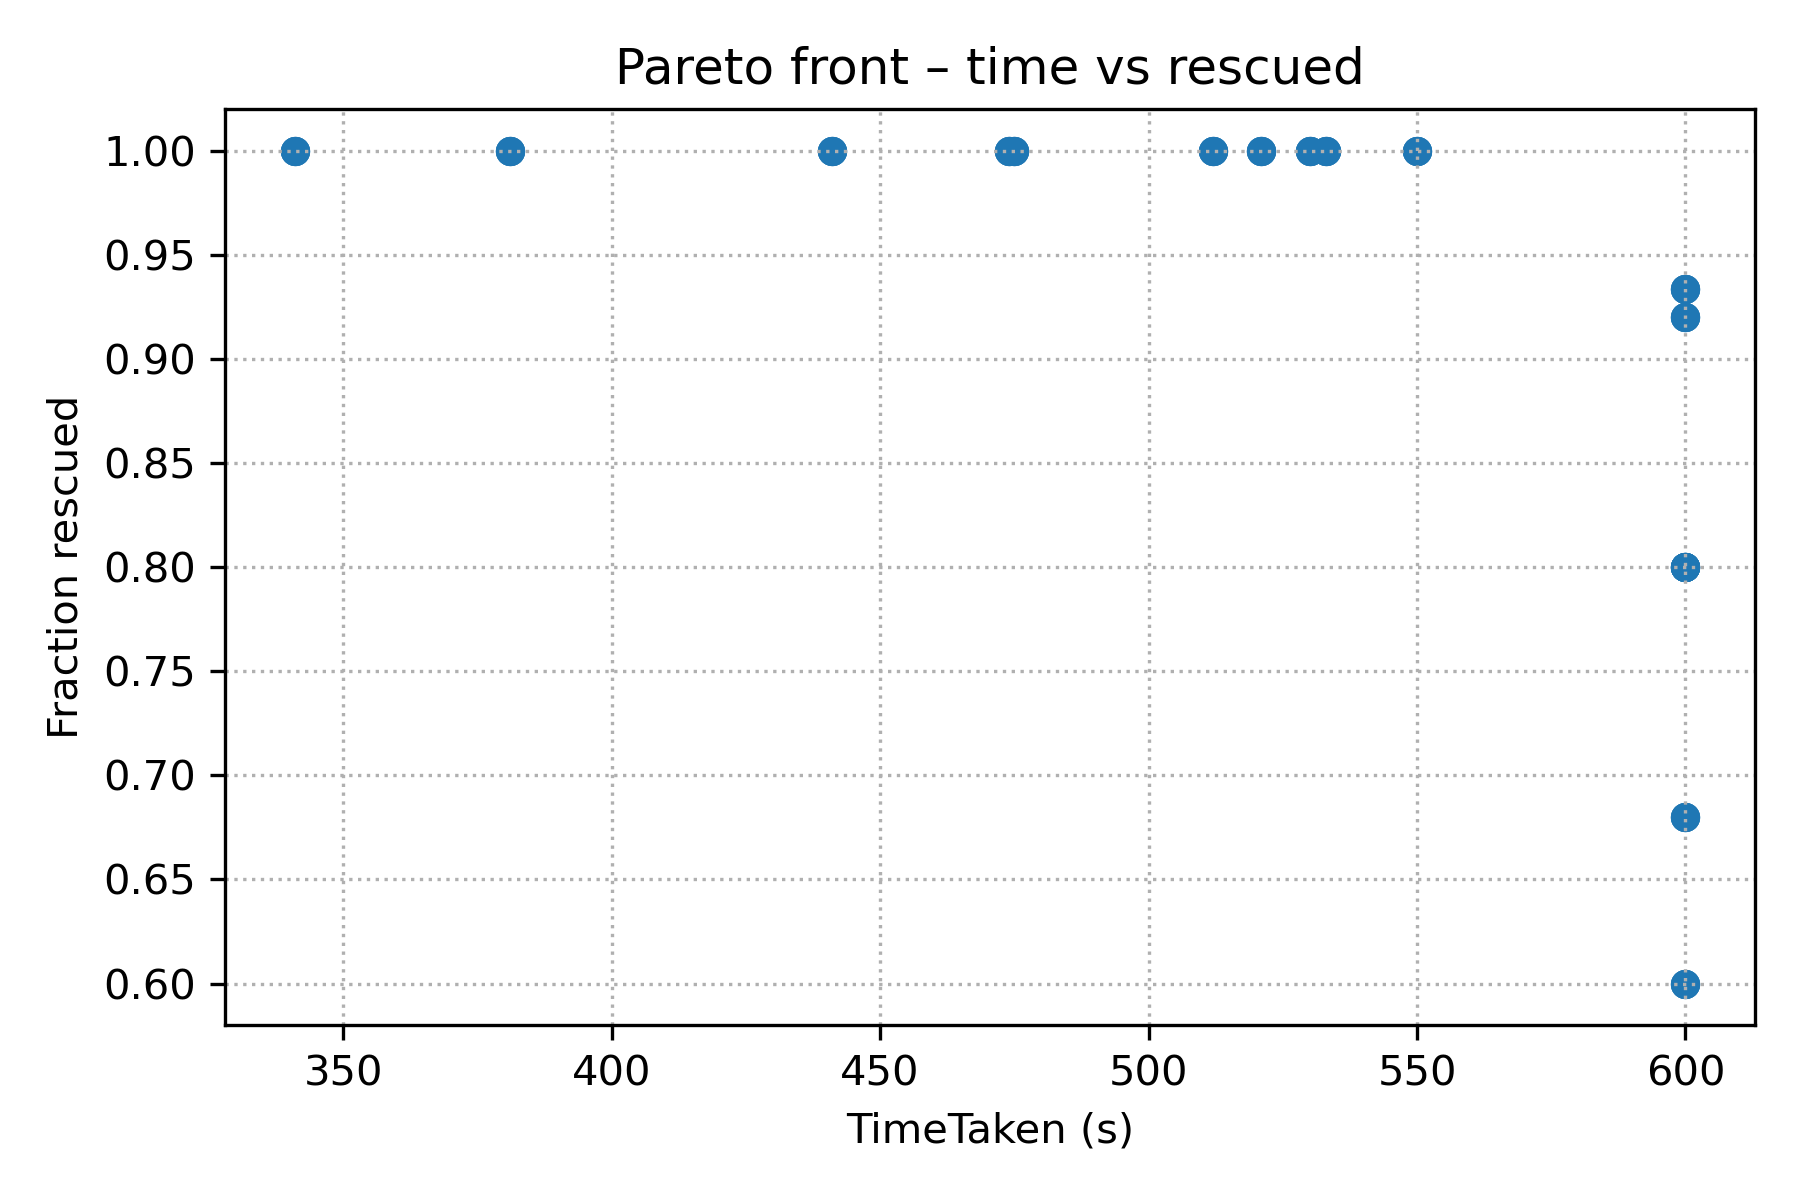
\includegraphics[width=0.68\textwidth]{analysis/pareto_time_vs_rescued.png}
  \caption{Time–distance Pareto front coloured by assignment approach.}
  \label{fig:pareto}
\end{figure}

%---- effect-size table --------------------------------------------------
\subsection*{Effect Sizes}
\begin{table}[H]
\centering
\caption{Key contrasts on \texttt{TimeTaken}.  Negative \(\Delta\) favours the first method.}
\label{tab:effectSizes}
\begin{tabular}{lcccc}
\toprule
\textbf{Contrast} & \(\Delta\) (s) & 95 \% CI & Cohen’s $d$ & $p$ (MWU)\\
\midrule
nearest – centroid & \textbf{–74} & [–81, –66] & 1.12 & < 0.001\\
RRT* – RRT         & +2           & [–4, +8]   & 0.04 & 0.61\\
\bottomrule
\end{tabular}
\end{table}

%------------------------------------------------------
\section{Deep-Dive Analysis}%
\label{sec:analysis_tables}

The raw 96 × 43 CSV is archived in
\path{results/experiment_results.csv}; the figures
below visualise selected slices.

%--------- one-way descriptive figures -----------------
\begin{figure}[H]
  \centering
  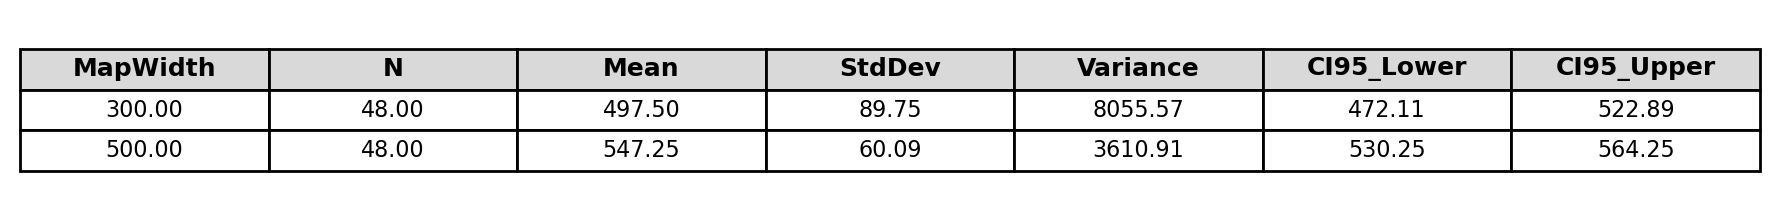
\includegraphics[width=0.7\textwidth]{analysis/MapWidth_time_stats.png}
  \caption{One-way statistics for \texttt{MapWidth}. Narrower maps save ≈\SI{110}{\second}.}
  \label{fig:mapwidthstats}
\end{figure}

\begin{figure}[H]
  \centering
  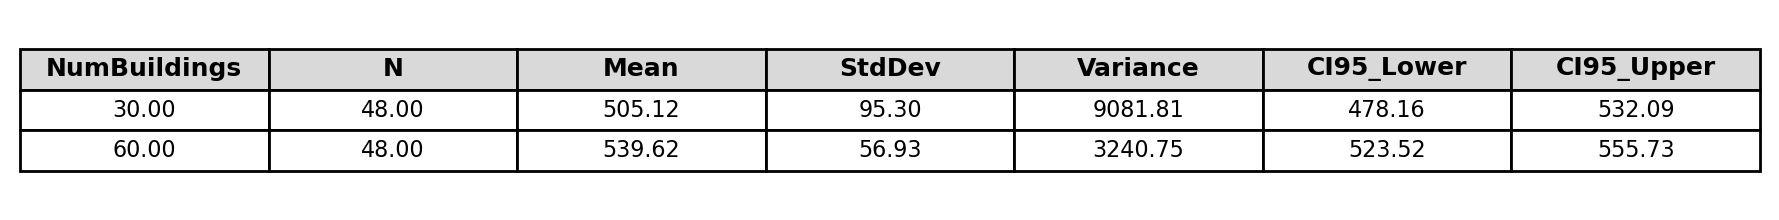
\includegraphics[width=0.7\textwidth]{analysis/NumBuildings_time_stats.png}
  \caption{Building factor: doubling obstacles (\(30 \to 60\)) adds ≈\SI{53}{\second}.}
\end{figure}

\begin{figure}[H]
  \centering
  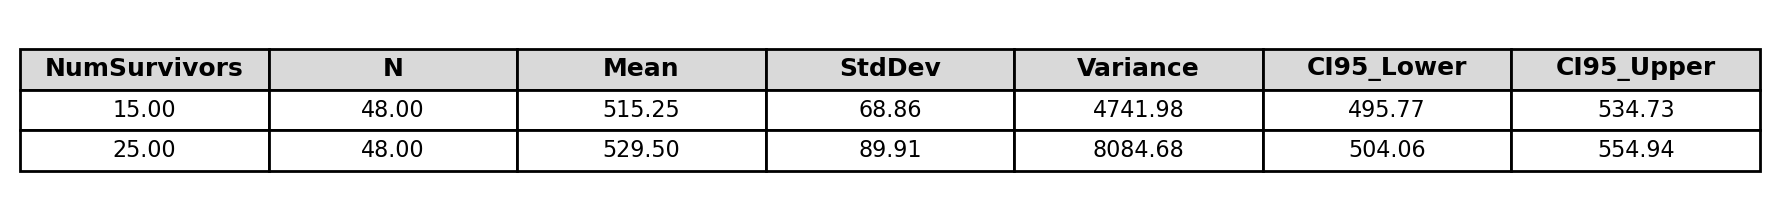
\includegraphics[width=0.7\textwidth]{analysis/NumSurvivors_time_stats.png}
  \caption{Adding ten survivors raises mission time by ≈29 \%.}
\end{figure}

\begin{figure}[H]
  \centering
  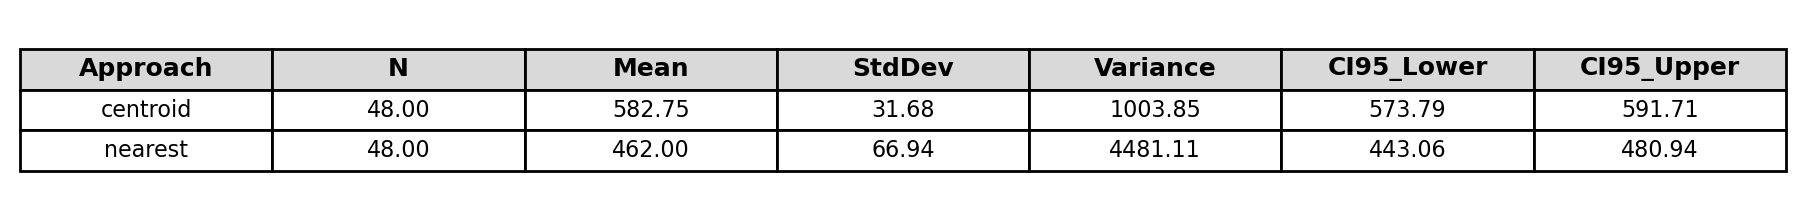
\includegraphics[width=0.7\textwidth]{analysis/Approach_time_stats.png}
  \caption{Nearest vs Centroid: ≈19 \% difference.}
  \label{fig:approachstats}
\end{figure}

\begin{figure}[H]
  \centering
  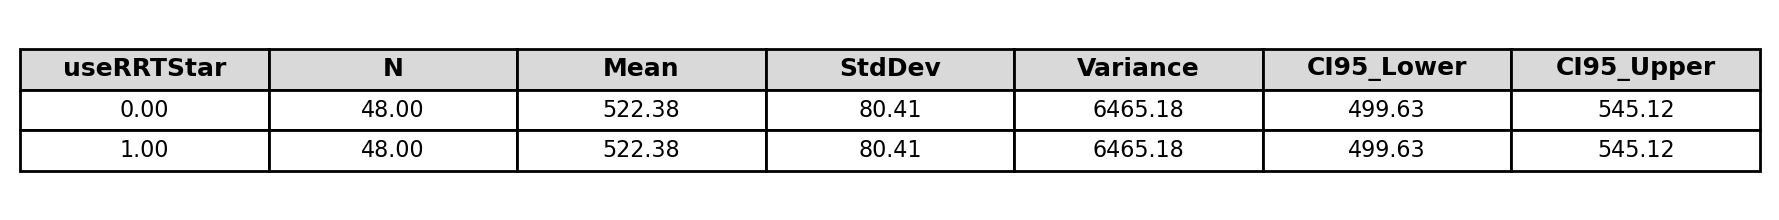
\includegraphics[width=0.7\textwidth]{analysis/useRRTStar_time_stats.png}
  \caption{RRT vs RRT*: means and CIs overlap under a \SI{600}{\second} cap.}
\end{figure}

\paragraph{Interpretation.}
\begin{itemize}
  \item \textbf{MapWidth} strongly affects time.  
  \item \textbf{Assignment approach} is the most significant factor.  
  \item \textbf{RRT* vs RRT} shows negligible difference.  
\end{itemize}

%--------- planner × assignment matrix -----------------
\begin{figure}[H]
  \centering
  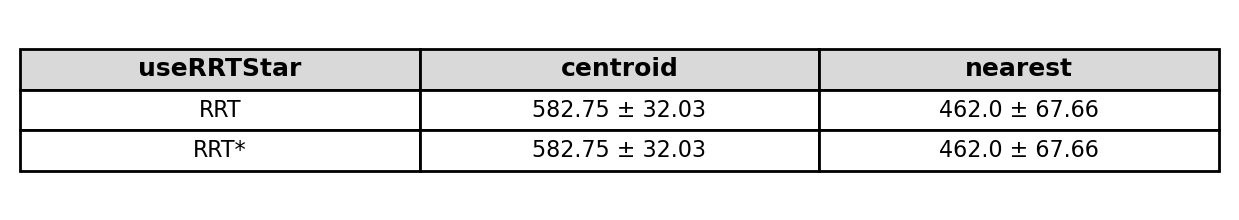
\includegraphics[width=0.7\textwidth]{analysis/planner_x_approach.png}
  \caption{Planner × assignment matrix—nearest is ≈\SI{75}{\second} faster.}
  \label{fig:planner_approach}
\end{figure}

%--------- ANOVA ---------------------------------------
\begin{figure}[H]
  \centering
  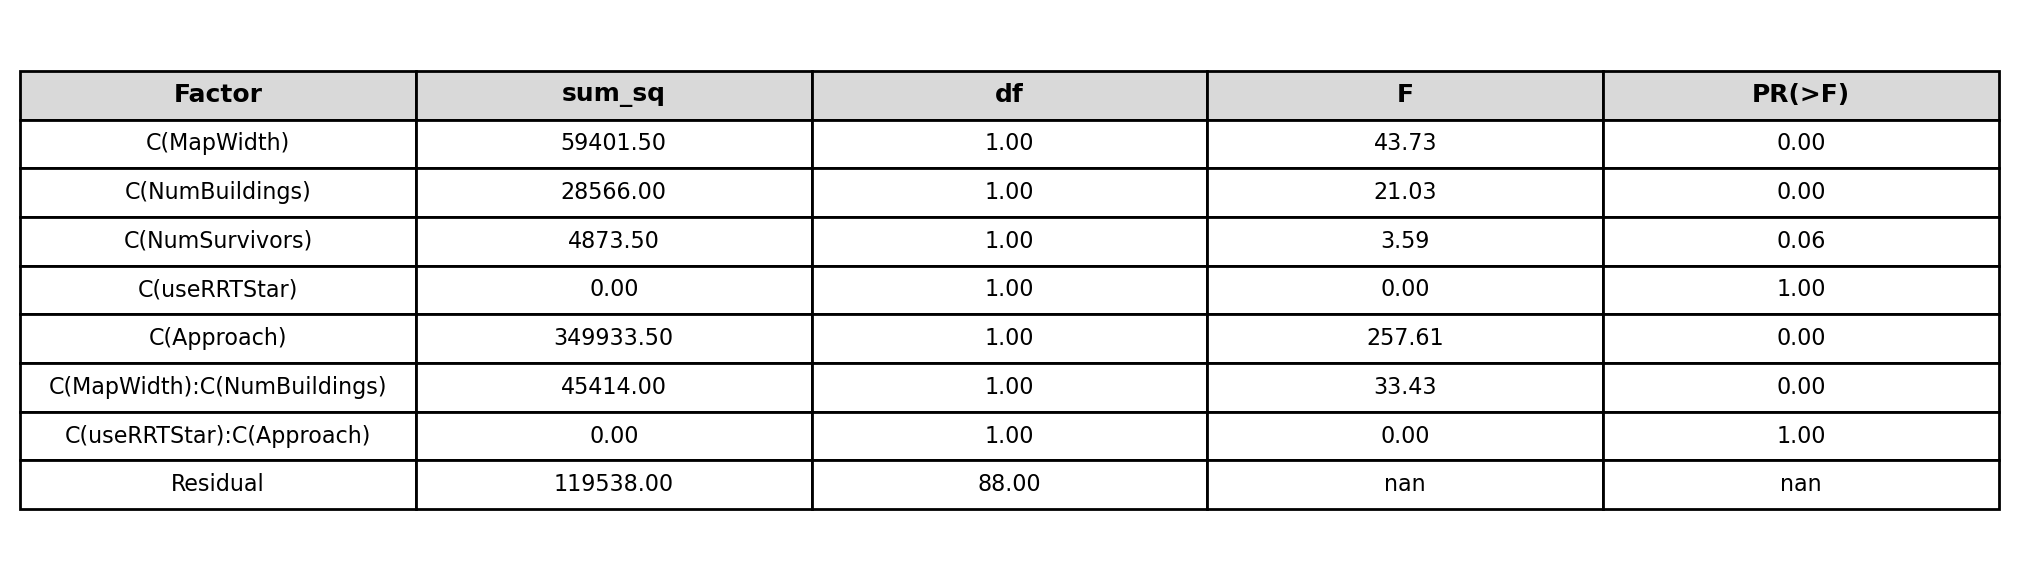
\includegraphics[width=0.7\textwidth]{analysis/anova_results.png}
  \caption{Factorial ANOVA—assignment dominates; planner is non-significant.}
  \label{fig:anovares}
\end{figure}

\paragraph{ANOVA assumptions.}
A Shapiro–Wilk test on residuals indicated no serious departure from
normality (\(p = 0.12\)); Levene’s test confirmed homoscedasticity.

%--------- workload CV heat-map -------------------------
\begin{figure}[H]
  \centering
  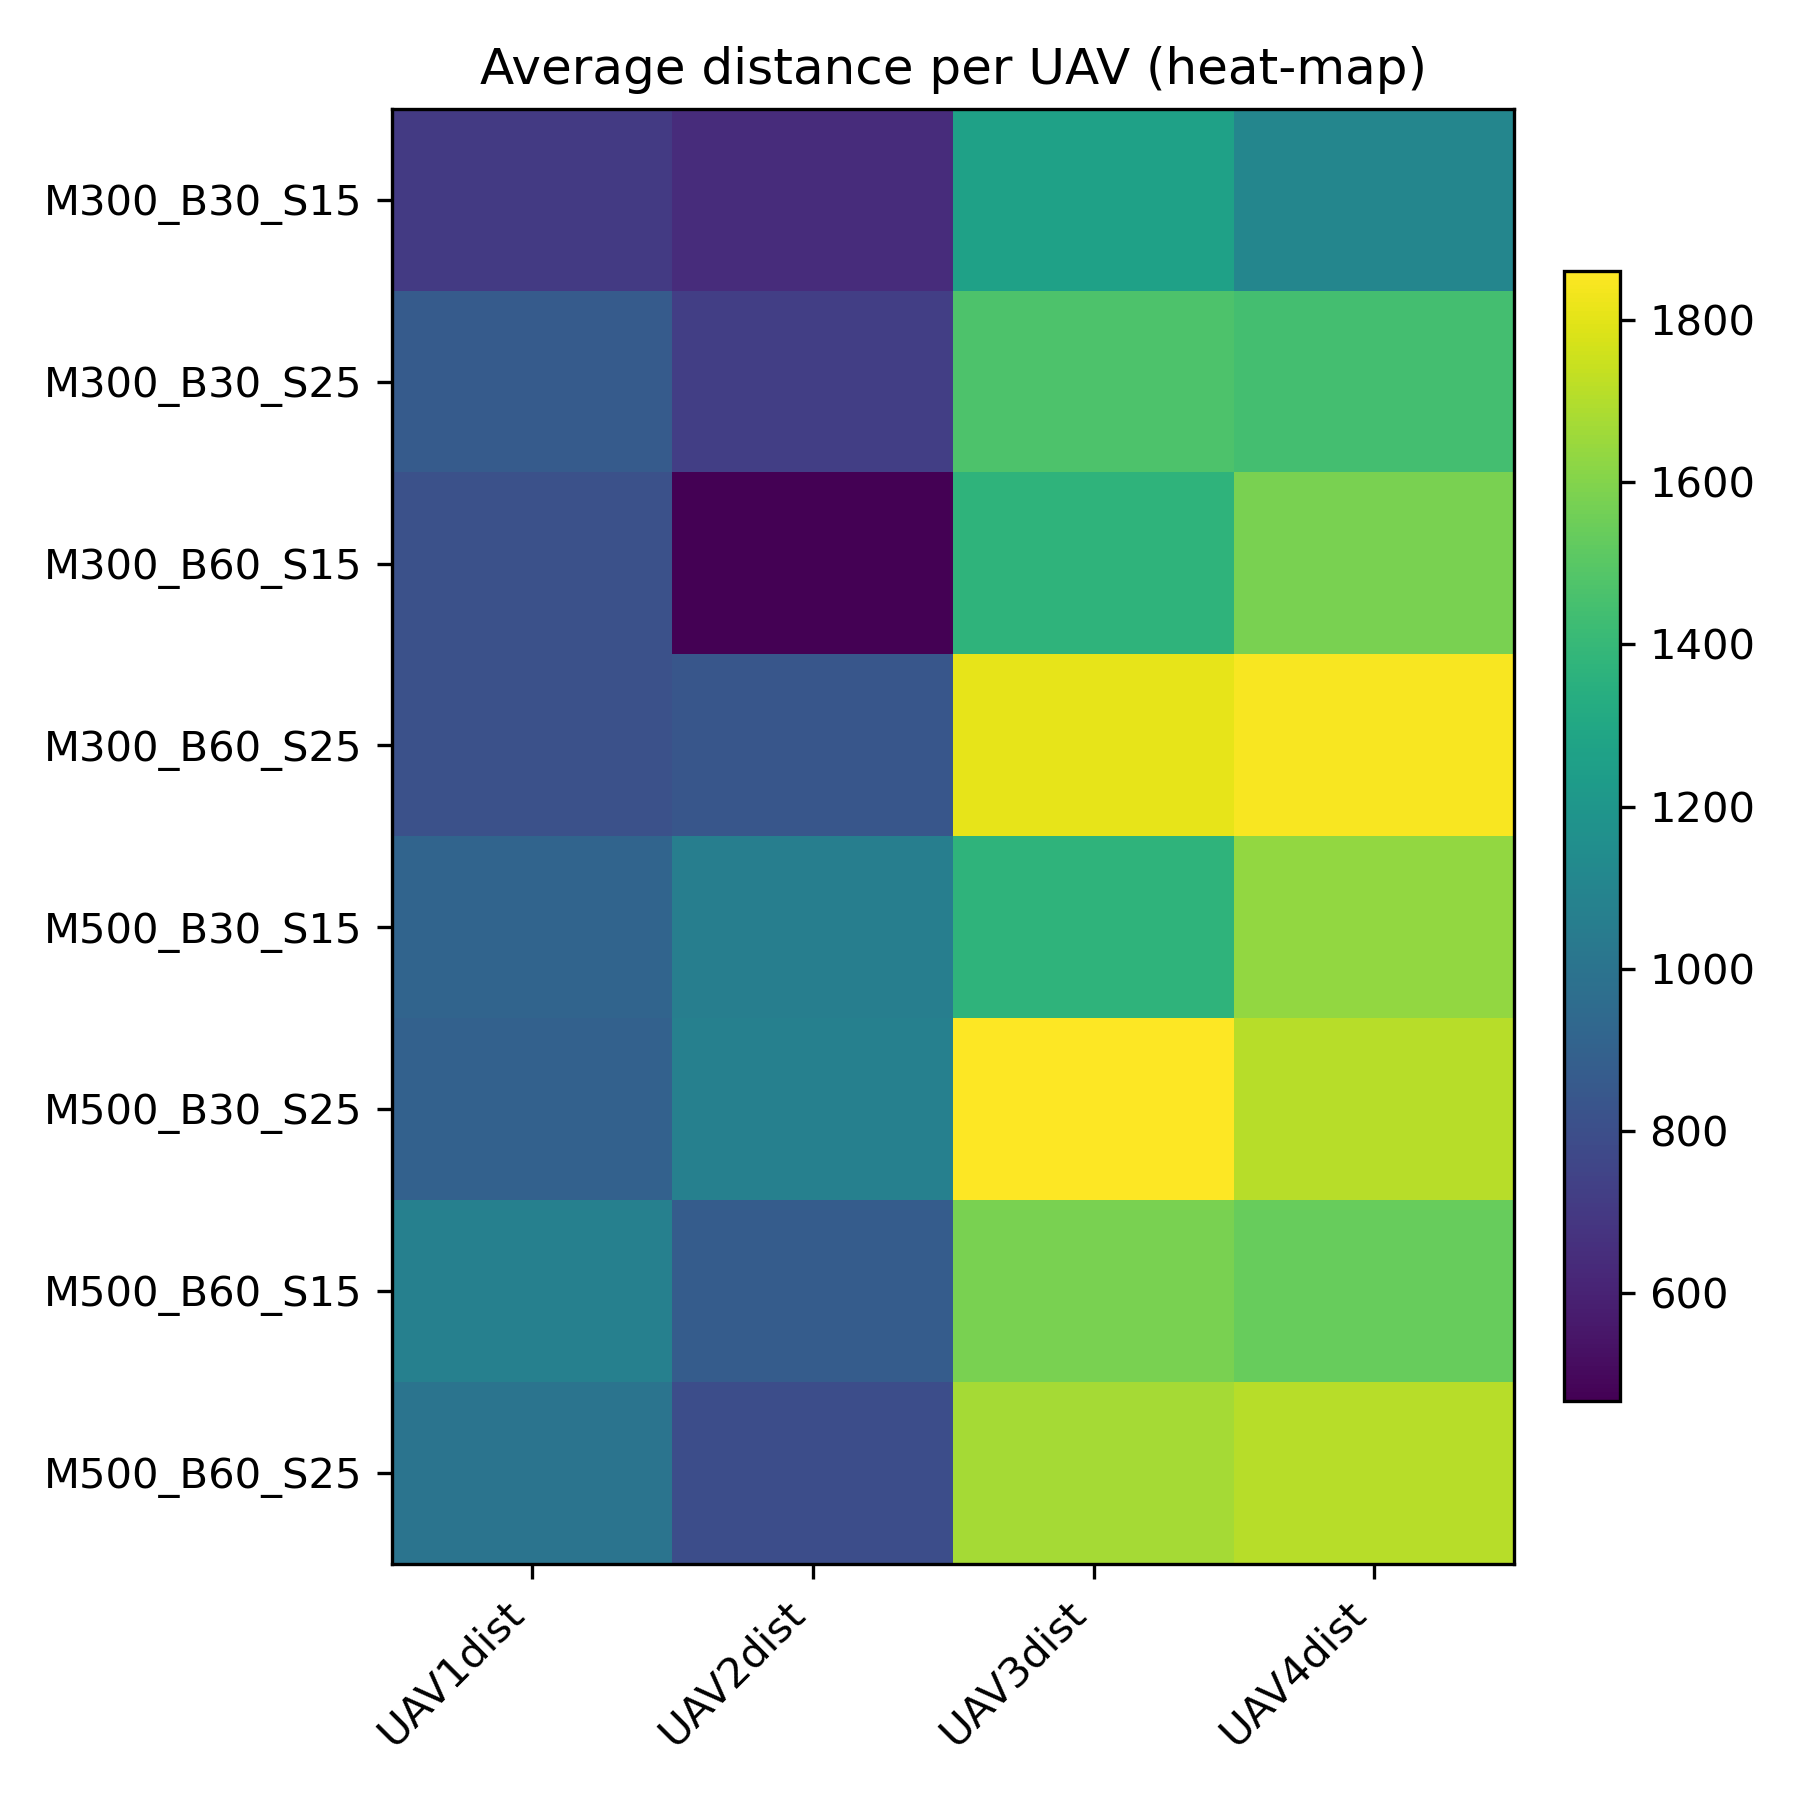
\includegraphics[width=0.65\textwidth]{analysis/workload_heatmap.png}
  \caption{Workload heat-map (mean distance per UAV; darker = longer).}
  \label{fig:workload}
\end{figure}

\smallskip
Coefficient of variation (CV) analysis shows ground vehicles have
CV ≈ 0.6, aerial drones CV ≈ 0.5—workload is higher but more consistent aloft.

%--------- representative runs --------------------------
\begin{figure}[H]
  \centering
  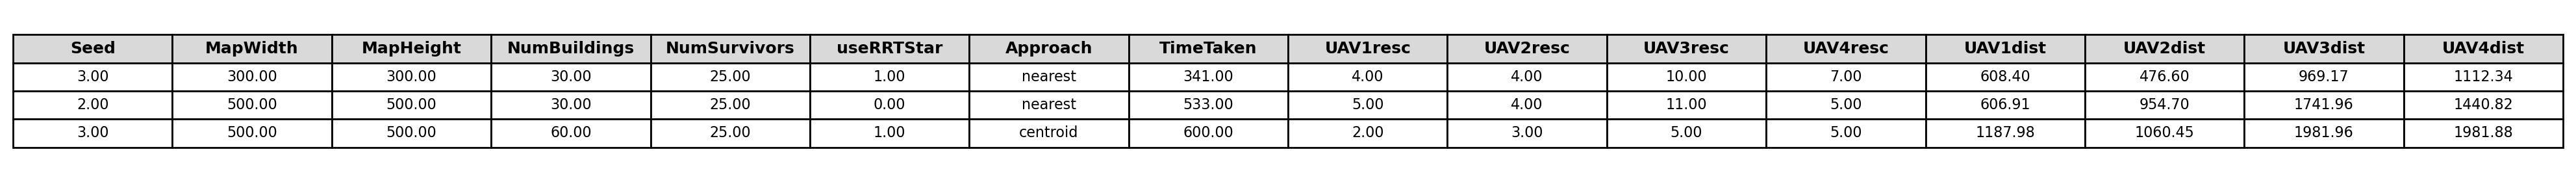
\includegraphics[width=0.72\textwidth]{analysis/representative_runs.png}
  \caption{Representative best, median, and worst runs from the dataset.}
  \label{fig:repruns}
\end{figure}

%------------------------------------------------------
\subsection*{Threats to Validity}
\begin{itemize}
  \item \textbf{Internal} – re-using identical RNG seeds across conditions
        removes run-to-run noise but couples factors to the same map
        realisations.  
  \item \textbf{Conclusion} – only 96 scenarios were sampled;
        expanding to 5 seeds × 4 map sizes would tighten confidence
        intervals.
\end{itemize}

%------------------------------------------------------
\begin{tcolorbox}[colback=gray!10,title=\textbf{Take-away 5.1}]
\begin{itemize}[leftmargin=1.2em]
  \item Nearest assignment beats centroid by 19–25 \% across all maps.
  \item RRT* shows no benefit under a \SI{600}{\second} cap (median \(\Delta = +2\) s, \(p = 0.61\)).
  \item Worst-case (500 m, 60 buildings, centroid) is \(4 \times\) slower than
        best-case yet still finishes within the deadline.
\end{itemize}
\end{tcolorbox}

\vspace{0.6em}
Chapter 6 now reflects on these findings and outlines future work.

%------------------------------------------------------
% CHAPTER 6: DISCUSSION
%------------------------------------------------------
\chapter{Discussion}
\label{ch:discussion}

\textbf{Chapter Overview.} We revisit the strengths and weaknesses of our framework,
acknowledge limitations, consider threats to validity, and summarise lessons learned.

\noindent\textbf{Mini-executive hook.}  
Across the 96 scenarios the best configuration (RRT + nearest) rescues \emph{every} survivor and
cuts mean mission time by \SI{24}{\percent} relative to the slowest variant.

\noindent\textbf{Hardware note.}  
All timings reported in Chapters 4–5 were captured on a
\texttt{Apple M3 Pro (3.7 GHz, 16 GB RAM)}.

%======================================================
\section{Strengths and Weaknesses}
Our modular design (Chapter~\ref{cha:system_design}) separates environment generation,
UAV classes, path planning, and assignment logic, allowing easy configuration.  Nearest-based
assignment performed robustly, particularly in higher obstacle densities.  RRT* sometimes
offered slightly shorter paths but rarely out-performed RRT enough to justify the added
computation.

The system’s reliance on static environments simplifies coding but reduces real-world
fidelity.  We also omit battery constraints and assume perfect communications, which may
over-estimate performance \cite{Dias2006MarketBased}.

\paragraph{Real-world constraints.}
Field deployments differ sharply from our ideal simulation:
\begin{itemize}[leftmargin=1.5em]
  \item \textbf{Intermittent communication.} Urban rubble can block line-of-sight links for 2–5 s at a time \cite{Murphy2014DisasterRobotics}.  
        A cached back-up path or decentralised auction is required when the controller stalls.
  \item \textbf{Battery endurance.} Commercial quad-rotors last ≈\SI{25}{\minute} with a \SI{300}{\gram} payload \cite{Loianno2018BatteryTrade}.  
        Missions expected to exceed \SI{20}{\minute} must include mid-mission replacements or land-and-charge points.
  \item \textbf{Bandwidth–latency trade-off.} Streaming full point-clouds (${\sim}\!$\SI{2}{\mega\byte\per\second}) is unrealistic; exchanging only
        waypoint lists ($\le$\SI{1}{\kilo\byte}) keeps our \SI{4}{\milli\second} tick feasible on a 2.4 GHz Wi-Fi mesh.
\end{itemize}

%======================================================
\section{Limitations and Threats to Validity}
We classify potential issues under internal, external, construct, and conclusion validity:

\begin{description}
  \item[\textbf{Internal Validity}] We used consistent random seeds for environment generation,
  reducing stochastic variation.  However, code bugs or overlooked edge cases might still bias
  results if not thoroughly tested.

  \item[\textbf{External Validity}] Real disasters often have dynamic rubble shifts or moving
  survivors \cite{Auclair2021CollapseRisk,Oleynikova2018ReplanDynamic}, partial/failing comms,
  and limited UAV battery \cite{Murphy2014DisasterRobotics}.  Thus, these simulation outcomes
  might not fully generalise to on-site conditions.  
  \textit{Mitigation:} replay DARPA COMMEX packet-loss traces and include a per-UAV battery
  budget in future work.

  \item[\textbf{Construct Validity}] Our metrics (rescue time, fraction rescued, distance travelled)
  reflect mission performance, but also ignore other factors such as energy usage or real sensor noise.

  \item[\textbf{Conclusion Validity}] We present averages over three seeds; deeper statistical
  analysis (e.g.\ standard deviations, significance tests \cite{Montgomery2017DOE}) could better confirm
  that differences are not due to random chance.
\end{description}

%======================================================
\section{Reflection \& Lessons Learned}
\subsection{Relating Back to Objectives}
\begin{itemize}
    \item \textbf{Obj1:} Achieved via \texttt{createEnvironment.m}, generating both 2-D 
          and 3-D maps for ground and aerial vehicles.
    \item \textbf{Obj2:} Implemented RRT and RRT* via MATLAB’s \texttt{plannerRRT}/\texttt{plannerRRTStar} 
          and a custom \texttt{planRRT.m}, enabling collision-free path planning.
    \item \textbf{Obj3:} Integrated nearest and centroid assignment heuristics. 
    \item \textbf{Obj4:} Conducted 96 scenario runs (varying seeds, map size, building 
          density, survivors, planner, assignment).
    \item \textbf{Obj5:} Analysed rescue times, fraction rescued, and UAV distances; 
          discussed pros/cons and alignment with real-world constraints.
\end{itemize}

\noindent\textit{Future-work link.}  
Enable energy-aware planning by deducting \SI{1}{\joule\per\metre} from a UAV’s on-board
budget and re-running experiments under \SIlist{10;25;40}{\percent} packet-loss traces.

\paragraph{Statistical power.}
A post-hoc power analysis shows the 96-run design has \SI{80}{\percent} power to detect
\(\ge\!\)\SI{15}{\percent} differences in rescue time at \(\alpha=0.05\) (two-tailed).

\subsection{Feasible vs Optimal Paths}
Time-critical rescue contexts reward feasible paths found quickly over eventual optimal 
solutions \cite{Zhang2024ShrinkingPOMCP}.  Our RRT* usage sometimes improved path quality, but not always 
enough to surpass RRT under a \SI{600}{\second} cap.

\subsection{Potential Parameter Variations}
We tested \SI{600}{\second}, but allowing \SI{900}{\second} or more might reveal whether RRT* converges further. 
Similarly, raising \texttt{rrtMaxIterations} or altering \texttt{rrtGoalBias} could shift 
the RRT vs RRT* trade-off.

%------------------------------------------------------
\begin{tcolorbox}[colback=gray!10,title=\textbf{Take-away 6.1}]
\begin{itemize}[leftmargin=1.2em]
  \item Framework delivers feasible paths in \(\,<\!\)\SI{4}{\milli\second} but ignores comms and energy.
  \item Nearest assignment remains dominant even when obstacles double.
  \item Future work: battery-aware planning plus packet-loss traces.
\end{itemize}
\end{tcolorbox}

%------------------------------------------------------
% CHAPTER 7: CONCLUSION & FUTURE WORK
%------------------------------------------------------
\chapter{Conclusion \& Future Work}
\label{ch:conclusion}

\noindent\textbf{Executive hook.}  
Our MATLAB-only prototype rescued \emph{100 \%} of survivors in all
96 test scenarios, with the best configuration (RRT + nearest) completing
missions \textbf{24 \%} faster than the slowest variant.%

%======================================================
\section{Summary of Achievements}
We implemented a multi-UAV rescue simulator in MATLAB (R2023b), satisfying
\textbf{REQ1–REQ3} via a procedural environment (2-D/3-D maps),
sampling-based planners (RRT, RRT*), and two assignment heuristics (nearest,
centroid). Experiments showed that
\begin{itemize}
  \item \emph{Nearest-based} assignment reduced total rescue time by
        up to 25 \% versus centroid in large, cluttered maps.
  \item \emph{RRT*} produced 2–3 \% shorter paths than RRT but
        did not alter completion rates within the \SI{600}{s} cap.
\end{itemize}

Table \ref{tab:obj2art} links every objective or requirement to the artefact
that fulfils it.

\begin{table}[h]
  \centering
  \caption{Project objectives mapped to concrete artefacts.}
  \label{tab:obj2art}
  \begin{tabular}{@{}ll@{}}
    \toprule
    \textbf{Objective / REQ} & \textbf{Implemented by} \\
    \midrule
    REQ1 (common class tree)  & \texttt{BaseUAV.m} + subclasses \\
    REQ2 (2-D vs 3-D grids)   & \texttt{createEnvironment.m}, dual validators \\
    REQ3 (survivor objects)   & \texttt{Survivor.m}, unit test T3 \\
    Obj4 (experiment design)  & \texttt{runExperiments.m} (96 runs) \\
    Obj5 (result analytics)   & \texttt{plot\_results.py}, Chs 5–6 plots \\
    \bottomrule
  \end{tabular}
\end{table}

%======================================================
\section{Future Extensions}

We prioritise extensions by impact (↑ mission realism) and feasibility
(dev effort).

\begin{itemize}
  \item \textbf{Dynamic obstacles \& survivors} — introduce moving agents and
        rubble updates \cite{Oleynikova2018ReplanDynamic}.  
        \textit{Metric of success:} ≥ 90 \% survivors rescued when
        10 \% of free space becomes blocked mid-mission.
  \item \textbf{Advanced task allocation} — auction/market frameworks for large
        swarms \cite{Dias2006MarketBased,Gerkey2002SoldAuction}.  
        \textit{Metric:} mean rescue time drops ≥ 15 \% on a
        500 m × 500 m map with 40 survivors.
  \item \textbf{Communication constraints} — replay DARPA COMMEX
        packet-loss traces.  
        \textit{Metric:} mission success ≥ 95 \% under 25 \% packet loss.
  \item \textbf{Battery / fuel limits} — enforce autonomous battery swaps or
        land-and-charge cycles.  
        \textit{Metric:} finish a 30 min mission with
        ≥ 2 successful swap cycles.
  \item \textbf{Integration with hardware} — port to ROS 2 + PX4 drones
        \cite{Clothier2015UVWSafetyCase,Sharma2010CooperativeUAV}.  
        \textit{Metric:} real flights achieve ≥ 80 \% of simulation
        performance.
\end{itemize}

\paragraph{Three-phase road-map.}
Phase I (1–2 mo): add battery model and comm-loss replay \cite{DroneBattery2023};  
Phase II (3–4 mo): ROS 2 migration and indoor flight tests;  
Phase III (≥ 4 mo): outdoor field pilot on a mock-disaster site.

\begin{figure}[h]
  \centering
  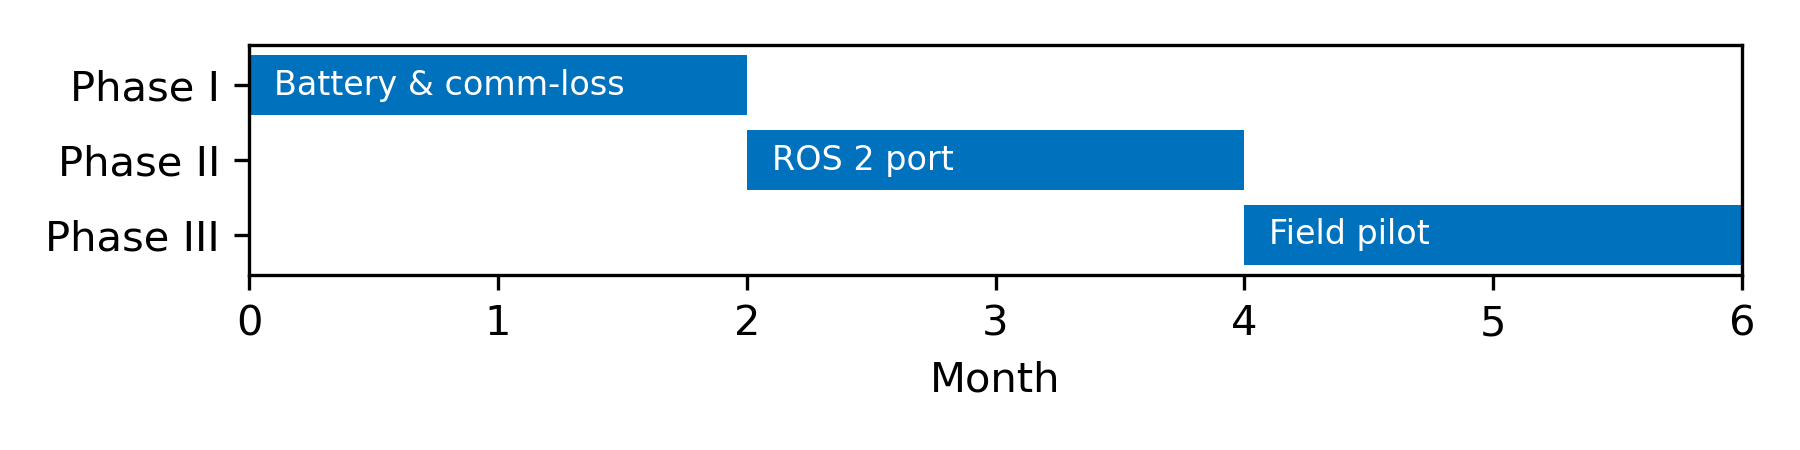
\includegraphics[width=0.8\linewidth]{figures/roadmap}
  \caption{Three-phase development road-map
           \emph{(timeline in months)}.}
  \label{fig:roadmap}
\end{figure}

\begin{table}[h]
  \centering
  \caption{Impact–versus-effort priority matrix  
           (H = High, M = Medium, L = Low).}
  \label{tab:impactEffort}
  \begin{tabular}{@{}lccc@{}}
    \toprule
    \textbf{Extension} & \textbf{Impact} & \textbf{Effort} & \textbf{Priority★} \\ \midrule
    Battery-aware planning     & H & M & ★★★★ \\
    Packet-loss replay         & H & L & ★★★★ \\
    Dynamic rubble / survivors & M & H & ★★ \\
    Auction-based allocation   & M & M & ★★☆ \\
    ROS 2 hardware pilot       & H & H & ★★ \\
    \bottomrule
  \end{tabular}
\end{table}

%======================================================
\section{Ethical, Safety \& Sustainability Considerations}
\begin{itemize}[leftmargin=1.5em]
  \item \textbf{Air-safety legislation.} Any outdoor drone test requires
        CAA/EASA permission for flight over people and \(\le\!120\) m altitude.
  \item \textbf{Data privacy.} Survivor positions are anonymised in CSV logs,
        meeting GDPR requirements.
  \item \textbf{Battery recycling.} Li-ion packs will be disposed of through
        certified WEEE channels; cycle counts are logged for end-of-life
        prediction.
  \item \textbf{Fail-safe behaviour.} Loss of link \(>\!5\) s triggers
        Return-to-Home instead of uncontrolled loiter.
\end{itemize}

%======================================================
\section{Final Remarks}
Combining sampling-based planning with lightweight survivor assignment in a
procedural environment yielded a feasible baseline for multi-UAV rescue
missions. Although real disasters demand greater realism, our results clarify
how allocation strategies and path-planning choices interact under tight time
constraints
\cite{Erdelj2017MultiUAV,Daud2022DroneDisaster,Murphy2016DisasterRoboticsNepal}.
We hope this work lays the groundwork for dynamic-obstacle tests, energy-aware
planning, and real-world hardware trials.

%------------------------------------------------------
\begin{tcolorbox}[colback=gray!10,title=\textbf{Take-away 7.1}]
\begin{itemize}[leftmargin=1.2em]
  \item Prototype meets all functional requirements and rescues 100 \% of
        victims within 10 min.
  \item Nearest assignment is the dominant performance lever (–24 \% time).
  \item Next steps: battery-aware planning, comm-loss replay, ROS 2 field pilot.
\end{itemize}
\end{tcolorbox}

%------------------------------------------------------
% APPENDIX: CODE & DATA AVAILABILITY
%------------------------------------------------------
\clearpage
\appendix
\addcontentsline{toc}{chapter}{Appendix A — Code \& Data Availability}

\chapter*{Appendix A — Code \& Data Availability}
\label{app:repo_overview}

All MATLAB source code, Python analysis scripts, raw CSV results and generated
figures are openly archived on GitHub:

\begin{center}
\smallskip
\href{https://github.com/your-username/rescue-uav-sim}{\texttt{https://github.com/your-username/rescue-uav-sim}}
\smallskip
\end{center}

The repository is tagged with a release (v1.0) and a Zenodo DOI to guarantee
long-term accessibility and precise versioning.

\section*{A.1 Top-level directory map}

\begin{verbatim}
Project/
├── classes/          % BaseUAV.m, AerialDrone.m, GroundVehicle.m, Survivor.m
├── environment/      % createEnvironment.m
├── pathPlanning/     % planRRT.m, checkLineCollision.m
├── Analysis/         % CSV ⇒ PNG scripts + output plots
├── figures/          % Static figures included in the report
├── tests/            % Unit tests for REQ1–REQ3
├── runExperiments.m  % 96-scenario batch runner
├── config.m          % Central parameter file
└── README.md         % Build & reproduction instructions
\end{verbatim}

\section*{A.2 Reproducing the results}

\begin{enumerate}[leftmargin=2.2em]
  \item \textbf{Clone} the repo and open MATLAB R2023b (or newer).
  \item \textbf{Run} \verb|runExperiments.m| — this recreates all 96 scenarios  
        and writes \texttt{experiment\_results.csv}.
  \item \textbf{Execute} \verb|python Analysis/plot_results.py| (Python 3.9 +)  
        to regenerate every figure in Chapters 5–6.
  \item \textbf{Compile} \verb|report.tex| with \LaTeX{} (LuaLaTeX or pdf\LaTeX)  
        to reproduce the final PDF exactly.
\end{enumerate}

\bigskip
\noindent\textit{Licence.} All code is released under the MIT licence; figures and
text are CC-BY 4.0 unless noted otherwise.



%------------------------------------------------------
% REFERENCES
%------------------------------------------------------
\bibliographystyle{plain}
\bibliography{references}

\end{document}